\chapter{参数敏感性}
\label{chap:parametric-sensitivity}

一笔预算要分给两种投入。预算从$2$增加到$2.1$，最优的损失能下降多少？理想配置改变一点，最优配置又往哪里移动？这些问题里，变的不是求解过程，而是问题本身。

把新问题重新解一遍当然可以得到答案，但它只回答一个具体的数。我们还想知道：多一单位预算值多少钱，这个价钱在多大范围内可信，几个参数同时变化时不重新求解能否估计结果，以及什么时候这样的估计根本不成立。

本章区分两个输出。最优值是一个数，它的变化可以由对偶乘子给出对任意大小扰动都成立的下界，也可以由包络关系给出局部导数。最优解是一个向量，它的移动要把最优性条件看成方程，用隐函数定理求导，因而需要更强的条件。

第~\ref{sec:sens-problems}节先说清参数变化时比较的是什么对象。第~\ref{sec:sens-value}节研究最优值，第~\ref{sec:sens-solution}节研究最优解，全章用同一个预算二次问题来核对公式。局部导数并不总是存在，第~\ref{sec:sens-branches}节用可以手算的例子拆开三种失效的原因。第~\ref{sec:sens-computation}节讨论怎样计算这些导数，又怎样检验算出的导数可信。

\section{含参问题}
\label{sec:sens-problems}

参数变化之后，“解的变化”到底指什么？本节要先回答这个问题。参数一变，问题可能没有解，也可能有许多解，所以必须先把比较的对象定义清楚。

\paragraph{贯穿全章的预算二次例}
沿用第~\ref{chap:constrained-optimality}章的预算分配。两种投入的数量是$x_1$、$x_2$，它们非负，总量不超过预算$\tau$。理想配置是$(2,1)$，偏离理想配置按平方计算损失。于是得到问题
\begin{equation}
 \min_{\bm{x}\in\mathbb{R}^2}\ \frac12(x_1-2)^2+\frac12(x_2-1)^2
 \quad\text{s.t.}\quad x_1+x_2\leq\tau,\ \ x_1\geq0,\ \ x_2\geq0.
 \label{eq:sens-budget}
\end{equation}
为了和一般记号对应，把三条约束写成$g_1=x_1+x_2-\tau$、$g_2=-x_1$、$g_3=-x_2$，都要求不大于零，相应的乘子是$\lambda_1,\lambda_2,\lambda_3$。

这个问题有清楚的几何图景。目标的等高线是以理想点$\bm{c}=(2,1)$为圆心的同心圆，所以最优解就是可行三角形里离$\bm{c}$最近的点。预算线像一堵可以平移的墙，$\tau$增大时墙向外退，三角形变大。

图~\ref{fig:sens-budget-family}画出三个预算水平。$\tau=4$时墙退得很远，碗底$(2,1)$本身可行，没有约束起作用。$\tau=2$时碗底被挡在墙外，解落在预算线上的$(3/2,1/2)$。$\tau=0.5$时三角形很小，解被挤到角点$(0.5,0)$，预算和$x_2\geq0$同时起作用。

\begin{BookInlineFigure}
 \centering
 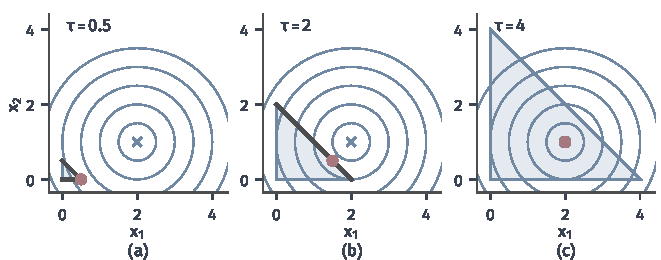
\includegraphics[width=112mm]{figures/05-optimization/06-constrained-optimization/matplotlib/sens-budget-family/figure.pdf}
 \caption{预算二次例~\eqref{eq:sens-budget}在三个预算下的情形。浅蓝三角形是可行集，蓝色同心圆是目标等高线，蓝色叉是理想点$(2,1)$，红点是最优解，深灰粗线是起作用的约束。(a)~$\tau=0.5$，预算和$x_2\geq0$都起作用。(b)~$\tau=2$，只有预算起作用。(c)~$\tau=4$，没有约束起作用。}
 \label{fig:sens-budget-family}
\end{BookInlineFigure}

\paragraph{变量与参数}
式~\eqref{eq:sens-budget}里有两类量。$\bm{x}$由优化决定，$\tau$由外部给定，求解时保持不变。前者是我们的选择，后者是我们所处的环境。同一个量算变量还是参数，取决于建模时想回答什么：若预算也可以选择，它就应该成为变量。

把环境写成参数向量$\bm{\theta}$，每个$\bm{\theta}$确定一个优化问题，全体构成一族问题。研究这族问题，需要两个输出对象。

\begin{definition}[含参问题、最优值函数与解映射]
\label{def:sens-family}
设$\bm{\Theta}\subseteq\mathbb{R}^q$是参数集合。对每个$\bm{\theta}\in\bm{\Theta}$，给定可行集$\bm{C}(\bm{\theta})\subseteq\mathbb{R}^n$和目标$f(\cdot,\bm{\theta})$，称
\begin{equation}
 \min_{\bm{x}\in\bm{C}(\bm{\theta})}f(\bm{x},\bm{\theta})
 \label{eq:sens-family}
\end{equation}
为\term{含参问题}（parametric problem）。函数
\begin{equation}
 V(\bm{\theta})=\inf_{\bm{x}\in\bm{C}(\bm{\theta})}f(\bm{x},\bm{\theta})
 \label{eq:sens-value}
\end{equation}
称为\term{最优值函数}（value function），并约定空集上的下确界为$+\infty$。把每个参数对应到最优解集合的映射
\begin{equation}
 \bm{S}(\bm{\theta})=\bigl\{\bm{x}\in\bm{C}(\bm{\theta}):f(\bm{x},\bm{\theta})=V(\bm{\theta})\bigr\}
 \label{eq:sens-solution-map}
\end{equation}
称为\term{解映射}（solution map）。
\end{definition}

$V$和$\bm{S}$的性格很不一样。$V(\bm{\theta})$总是一个确定的量，只是可能取$\pm\infty$。$\bm{S}(\bm{\theta})$是一个集合，可能是空集，可能只有一个点，也可能有无穷多个点。对预算例，$\tau<0$时可行集是空集，所以$V(\tau)=+\infty$，$\bm{S}(\tau)=\varnothing$。$\tau\geq0$时目标强凸、可行集紧，$\bm{S}(\tau)$恰有一个点。

\paragraph{参数改变可能使问题失去解}
除了不可行，参数改变还可能让最小值取不到。下面的一族问题定义在整条实轴上：
\[
 \min_{x\in\mathbb{R}}\ f(x,\theta)=e^{x}-\theta x.
\]
图~\ref{fig:sens-three-outcomes}画出三种情况，下面逐个计算。

\begin{BookInlineFigure}
 \centering
 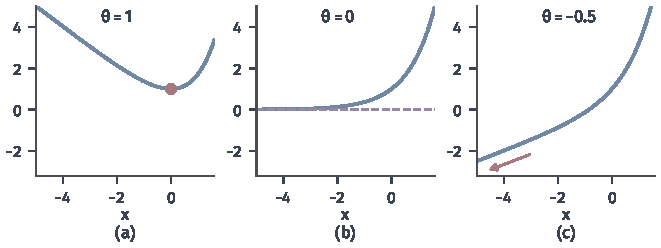
\includegraphics[width=112mm]{figures/05-optimization/06-constrained-optimization/matplotlib/sens-three-outcomes/figure.pdf}
 \caption{同一族目标$f(x,\theta)=e^{x}-\theta x$在三个参数下的结果。(a)~$\theta=1$，最小值$1$在红点$x=0$取得。(b)~$\theta=0$，下确界$0$（紫色虚线）有限但取不到。(c)~$\theta=-0.5$，红色箭头表示目标沿$x\to-\infty$无下界。}
 \label{fig:sens-three-outcomes}
\end{BookInlineFigure}

$\theta>0$时，令导数$e^x-\theta$为零，得到唯一的驻点$x=\ln\theta$。二阶导数$e^x$为正，所以它是全局极小点，并且
\[
 V(\theta)=\theta-\theta\ln\theta,\qquad \bm{S}(\theta)=\{\ln\theta\}.
\]

$\theta=0$时目标是$e^x$，它的下确界是$0$，但没有点取得这个值，所以$V(0)=0$而$\bm{S}(0)=\varnothing$。$\theta<0$时，$x\to-\infty$使$-\theta x=\lvert\theta\rvert x\to-\infty$，而$e^x\to0$，所以$V(\theta)=-\infty$。

这族问题还显示出值与解的差别。$\theta\downarrow0$时，$V(\theta)=\theta-\theta\ln\theta\to0=V(0)$，值的变化是连续的。解却是$\ln\theta\to-\infty$，一路跑向无穷远。讨论变化之前，必须先确认所研究的$\bm{\theta}$处解存在，并说明比较的是值还是解。

\paragraph{有多个解时要说清跟踪谁}
考虑一个有两个山谷的目标：
\begin{equation}
 f(x,\theta)=(x^2-1)^2+\theta x.
 \label{eq:sens-double-well}
\end{equation}
$\theta=0$时两个谷底$x=\pm1$同样低，$\bm{S}(0)=\{-1,1\}$。$\theta$不为零时，$\theta x$这一项把地面倾斜，一个谷底升高，另一个降低。“最优解对$\theta$的导数”这句话在$\theta=0$处没有明确含义，因为不知道说的是哪一个解。

这时有两种办法把问题说清楚。一种是跟踪一条\term{局部极小分支}（local minimizer branch），即在$\bm{\theta}_0$的邻域上定义的映射$\bm{x}(\bm{\theta})$，使每个$\bm{x}(\bm{\theta})$都是相应问题的局部极小点，并且随$\bm{\theta}$连续变化。另一种是约定\term{选解规则}（selection rule），例如总取最优解中范数最小的一个。

沿分支的目标值记作
\begin{equation}
 v(\bm{\theta})=f(\bm{x}(\bm{\theta}),\bm{\theta}).
 \label{eq:sens-branch-value}
\end{equation}
小写的$v$是某条分支上的值，大写的$V$是全局最优值。分支上的点都可行，所以$v(\bm{\theta})\geq V(\bm{\theta})$，只有分支恰好全局最优时才取等号。

图~\ref{fig:sens-double-well}展示了这种区别。(b)中两条绿色虚线是两个谷底的位置，它们各自光滑。红色实线是全局最优解，它在$\theta=0$处从上面一条跳到下面一条。(c)中分支的值光滑地穿过$\theta=0$，全局最优值是两者中较小的那个，在$\theta=0$处有折角。例如沿右侧谷底的分支在$\theta>0$时仍然是局部极小，但它的值已经高于全局最优值，不能称为“最优值”。

\begin{BookInlineFigure}
 \centering
 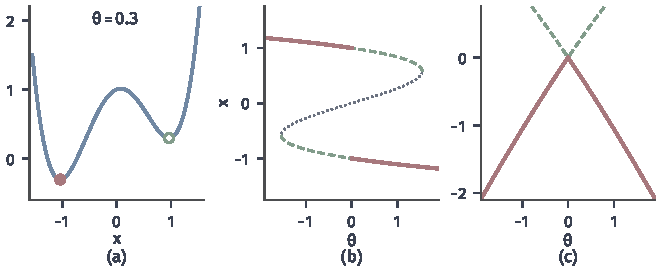
\includegraphics[width=112mm]{figures/05-optimization/06-constrained-optimization/matplotlib/sens-double-well/figure.pdf}
 \caption{双谷目标~\eqref{eq:sens-double-well}的分支与全局解。(a)~$\theta=0.3$时的目标，红点是全局最小点，绿色空心点是另一个局部极小点。(b)~驻点随$\theta$的变化：绿色虚线是局部极小分支，灰色点线是局部极大分支，红色实线是全局最优解。(c)~绿色虚线是两条分支上的目标值，红色实线是全局最优值。}
 \label{fig:sens-double-well}
\end{BookInlineFigure}

图~\ref{fig:sens-objects}汇总这些对象的关系。本章每个结论都会说明针对哪一个对象：是全局的$V$，还是某条分支上的$v$；是整个解集合$\bm{S}$，还是分支$\bm{x}(\bm{\theta})$。

\begin{BookInlineFigure}
 \centering
 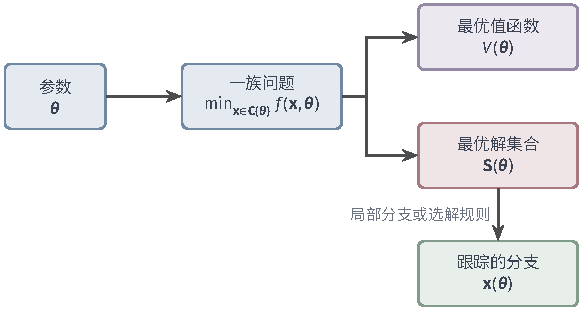
\includegraphics[width=99mm]{figures/05-optimization/06-constrained-optimization/tikz/sens-objects/figure.pdf}
 \caption{含参问题的三个输出对象。参数确定一个优化问题，问题确定最优值函数和最优解集合。解集合可能为空或含多个点，只有通过局部分支或选解规则，才得到一个随参数变化的点。}
 \label{fig:sens-objects}
\end{BookInlineFigure}

\section{最优值的变化}
\label{sec:sens-value}

参数变了以后，最优值变化多少？本节研究这个问题。先让约束的右端变化，乘子会给出一个对任意大小的扰动都成立的下界；再让目标和约束显含一般的参数，这时得到的是局部导数。“下界的斜率”“实际的导数”“方向导数”是三个不同的量，下面逐个说明它们各自成立的条件。

\subsection{约束右端的全局变化界}
\label{sec:sens-rhs-bound}

\paragraph{扰动右端}
对一般约束问题，在每条约束的右端加上扰动，定义
\begin{equation}
 V(\bm{u},\bm{v})=\inf\bigl\{f(\bm{x}):\ g_i(\bm{x})\leq u_i,\ h_j(\bm{x})=v_j,\ \forall i,j\bigr\}.
 \label{eq:sens-rhs-value}
\end{equation}
这里$\bm{u}\in\mathbb{R}^m$，$\bm{v}\in\mathbb{R}^p$，不可行时$V=+\infty$。基准问题的最优值是$f^\star=V(\bm{0},\bm{0})$。$u_i>0$把第$i$条不等式放宽，$u_i<0$把它收紧。

\paragraph{按旧价格结算}
第~\ref{chap:duality}章的Lagrange函数是
\[
 \mathcal{L}(\bm{x},\bm{\lambda},\bm{\nu})=f(\bm{x})+\sum_{i=1}^m\lambda_ig_i(\bm{x})+\sum_{j=1}^p\nu_jh_j(\bm{x}),
\]
对偶函数是
\[
 q(\bm{\lambda},\bm{\nu})=\inf_{\bm{x}}\mathcal{L}(\bm{x},\bm{\lambda},\bm{\nu}).
\]
弱对偶说$\bm{\lambda}\geq\bm{0}$时$q(\bm{\lambda},\bm{\nu})\leq f^\star$，强对偶且乘子达到则说存在$(\bm{\lambda}^\star,\bm{\nu}^\star)$，使$q(\bm{\lambda}^\star,\bm{\nu}^\star)=f^\star$。

可以把乘子想成一张事先定好的价格表：用$g_i(\bm{x})$这么多资源，就按$\lambda_i^\star$的单价结算。强对偶达到的意思是，在这张价格表下，每一个点$\bm{x}$的结算额$\mathcal{L}(\bm{x},\bm{\lambda}^\star,\bm{\nu}^\star)$都不低于$f^\star$。若右端变了，新问题的可行点仍然要按这张旧价格表结算，结算额的下限不变，由此就得到新最优值的下界。

\begin{theorem}[最优值的全局下界]
\label{thm:sens-rhs-bound}
设基准问题的最优值$f^\star$有限，存在$\bm{\lambda}^\star\geq\bm{0}$与$\bm{\nu}^\star$，使$q(\bm{\lambda}^\star,\bm{\nu}^\star)=f^\star$。则对所有$(\bm{u},\bm{v})\in\mathbb{R}^m\times\mathbb{R}^p$，
\begin{equation}
 V(\bm{u},\bm{v})\geq f^\star-\langle\bm{\lambda}^\star,\bm{u}\rangle-\langle\bm{\nu}^\star,\bm{v}\rangle.
 \label{eq:sens-rhs-bound}
\end{equation}
\end{theorem}

\begin{proof}
若扰动问题不可行，左端是$+\infty$，结论成立。否则任取扰动问题的可行点$\bm{x}$。由$q$的定义，
\[
 f^\star=q(\bm{\lambda}^\star,\bm{\nu}^\star)\leq\mathcal{L}(\bm{x},\bm{\lambda}^\star,\bm{\nu}^\star).
\]

把Lagrange函数展开。由$\lambda_i^\star\geq0$和$g_i(\bm{x})\leq u_i$，第$i$个不等式项不超过$\lambda_i^\star u_i$。由$h_j(\bm{x})=v_j$，等式项正好等于$\nu_j^\star v_j$。于是
\[
 f^\star\leq f(\bm{x})+\langle\bm{\lambda}^\star,\bm{u}\rangle+\langle\bm{\nu}^\star,\bm{v}\rangle.
\]
移项后对所有可行的$\bm{x}$取下确界，就得到式~\eqref{eq:sens-rhs-bound}。
\end{proof}

式~\eqref{eq:sens-rhs-bound}的右端是$(\bm{u},\bm{v})$的仿射函数，它在原点与$V$相等，在其他地方不超过$V$。第$i$条不等式方向上，下界的斜率是$-\lambda_i^\star$，负号来自“右端增大意味着约束放宽”。放宽$u_i>0$时，最优值至多下降$\lambda_i^\star u_i$。收紧$u_i<0$时，最优值至少上升$\lambda_i^\star\lvert u_i\rvert$。

\paragraph{条件各起什么作用}
定理没有要求问题是凸的，也没有要求函数可微，证明里只用了不等式。它也不要求扰动后的解和基准解有相同的活动约束，甚至不要求解存在。所以这是一个全局结论，对很大的扰动同样成立，只是方向是单侧的。

定理还有一个推论：在这些条件下，任何右端扰动都不会使问题变得无下界，因为式~\eqref{eq:sens-rhs-bound}的右端总是有限的。

\paragraph{预算例的验证}
取基准预算$\tau=2$，令$u=\tau-2$，只扰动第一条约束。基准解是$\bm{x}^\star=(3/2,1/2)$，后两条约束不起作用。乘子取$\bm{\lambda}^\star=(1/2,0,0)$，此时Lagrange函数是
\[
 \mathcal{L}(\bm{x},\bm{\lambda}^\star)=\frac12(x_1-2)^2+\frac12(x_2-1)^2+\frac12(x_1+x_2-2).
\]

这是关于$\bm{x}$的强凸二次函数。令梯度为零，得到$x_1-2+\tfrac12=0$与$x_2-1+\tfrac12=0$，极小点恰好是$(3/2,1/2)$。把它代入，因为$x_1+x_2-2=0$，所以
\[
 q(\bm{\lambda}^\star)=\frac12\cdot\frac14+\frac12\cdot\frac14=\frac14=f^\star.
\]

零间隙得到验证，强对偶和乘子达到都成立。式~\eqref{eq:sens-rhs-bound}于是给出：对所有$\tau$，
\begin{equation}
 V(\tau)\geq\frac14-\frac12(\tau-2).
 \label{eq:sens-budget-bound}
\end{equation}
下面在三个预算上核对。对$\tau=2.1$，解是$(1.55,0.55)$；对$\tau=0.5$，解是$(0.5,0)$；对$\tau=4$，解是$(2,1)$。三处的真实最优值和下界分别是
\[
 V(2.1)=0.2025\geq0.2,\qquad
 V(0.5)=1.625\geq1,\qquad
 V(4)=0\geq-0.75.
\]

预算从$2$增加到$2.1$时，最优值实际下降$0.0475$，下界说它至多下降$0.05$。注意$\tau=0.5$时活动约束已经和基准解不同，$\tau=4$时预算根本不起作用，下界依然正确。图~\ref{fig:sens-global-bound}画出整条曲线，紫色直线始终在蓝色曲线下方。

\begin{BookInlineFigure}
 \centering
 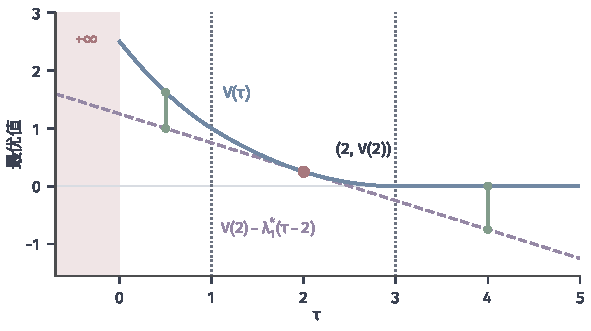
\includegraphics[width=100mm]{figures/05-optimization/06-constrained-optimization/matplotlib/sens-global-bound/figure.pdf}
 \caption{预算例的最优值函数（蓝线）和由$\tau=2$处乘子$\lambda_1^\star=1/2$给出的下界（紫色虚线）。红点是基准点，绿色线段是$\tau=0.5$和$\tau=4$处下界的余量，灰色点线标出活动约束改变的$\tau=1,3$。红色区域$\tau<0$不可行，$V=+\infty$。}
 \label{fig:sens-global-bound}
\end{BookInlineFigure}

\paragraph{去掉强对偶会怎样}
强对偶达到这个条件不能换成“存在KKT乘子”。考虑非凸问题
\[
 \min_{x\in\mathbb{R}}\ -x^2\quad\text{s.t.}\quad x-1\leq u,\ \ -x-1\leq0.
\]
基准问题$u=0$的可行集是$[-1,1]$，$f^\star=-1$，在$x=\pm1$取得。

在$x=1$处，平稳条件$-2x+\lambda_1=0$给出KKT乘子$\lambda_1=2$，第二条约束不起作用，$\lambda_2=0$。如果照搬式~\eqref{eq:sens-rhs-bound}，会得到$V(u)\geq-1-2u$。

直接计算最优值。$u>0$时可行集是$[-1,1+u]$，最小点在$x=1+u$。$-2\leq u\leq0$时，可行集右端点的绝对值不超过$1$，最小点在$x=-1$。所以
\[
 V(u)=\begin{cases}-1,&-2\leq u\leq0,\\-(1+u)^2,&u>0.\end{cases}
\]
$u>0$时，
\[
 V(u)-(-1-2u)=-u^2<0,
\]
下界不成立，见图~\ref{fig:sens-kkt-no-bound}。原因是这个问题的对偶函数对任何乘子都是$-\infty$，强对偶不成立。KKT乘子只承载局部信息，全局下界必须由对偶最优的乘子给出。

\begin{BookInlineFigure}
 \centering
 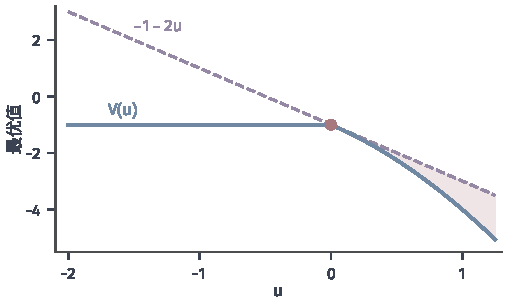
\includegraphics[width=86mm]{figures/05-optimization/06-constrained-optimization/matplotlib/sens-kkt-no-bound/figure.pdf}
 \caption{KKT乘子不给出全局下界的例子。蓝线是$\min-x^2$，$x-1\leq u$，$x\geq-1$的最优值$V(u)$，紫色虚线是用$x=1$处KKT乘子$2$写出的直线$-1-2u$，红色区域表示$u>0$时直线高于$V$。}
 \label{fig:sens-kkt-no-bound}
\end{BookInlineFigure}

非凸并不一定导致失败。对问题$\min-x^2$，$x^2-1\leq u$，取$\lambda=1$，Lagrange函数恒等于$-1$，所以$q(1)=-1=f^\star$。此时$V(u)=-1-u$（$u\geq-1$），下界恰好取等号。起决定作用的是零间隙，而不是凸性。

\subsection{乘子的边际解释}
\label{sec:sens-marginal}

下界只说明$V$不低于一条直线。什么时候这条直线就是$V$的切线，乘子就是最优值的真实变化率？本小节回答这个问题。

\paragraph{直线贴着曲线时}
一条直线处处不高于曲线，又在基准点与曲线相交。如果曲线在该点光滑，直线就没有选择，只能是切线。这正是图~\ref{fig:sens-global-bound}中红点处的情形。把这个几何观察写成定理：

\begin{theorem}[乘子是边际变化率]
\label{thm:sens-marginal}
在定理~\ref{thm:sens-rhs-bound}的条件下，进一步设$V$在$(\bm{0},\bm{0})$附近有限且在$(\bm{0},\bm{0})$可微，则
\begin{equation}
 \frac{\partial V}{\partial u_i}(\bm{0},\bm{0})=-\lambda_i^\star,
 \qquad
 \frac{\partial V}{\partial v_j}(\bm{0},\bm{0})=-\nu_j^\star.
 \label{eq:sens-marginal}
\end{equation}
\end{theorem}

\begin{proof}
定义函数
\[
 \varphi(\bm{u},\bm{v})=V(\bm{u},\bm{v})-f^\star+\langle\bm{\lambda}^\star,\bm{u}\rangle+\langle\bm{\nu}^\star,\bm{v}\rangle.
\]
式~\eqref{eq:sens-rhs-bound}说明$\varphi\geq0$，而$\varphi(\bm{0},\bm{0})=0$，所以原点是$\varphi$的极小点。原点是定义域的内点，$\varphi$在原点可微，它的梯度必须为零。写出这个梯度的各个分量，就是式~\eqref{eq:sens-marginal}。
\end{proof}

定理同时说明，只要$V$在基准点可微，满足条件的乘子就是唯一的，因为它们都等于$V$的梯度的相反数。

\paragraph{几何含义}
在预算例中，$-\nabla f(\bm{x}^\star)=\lambda_1^\star(1,1)$垂直于预算线。图~\ref{fig:sens-shadow-price-geometry}中，预算增加$\Delta\tau$时，预算线沿法向平移$\Delta\tau/\sqrt{2}$。目标沿法向的变化率是
\[
 \lVert\nabla f(\bm{x}^\star)\rVert_2=\lambda_1^\star\sqrt{2}.
\]
两者相乘，目标的一阶下降量是$\lambda_1^\star\Delta\tau$，这就是乘子作为\emph{影子价格}的含义：多一单位预算大约值$\lambda_1^\star$。没有起作用的约束乘子为零，放宽它们一阶没有价值。

\begin{BookInlineFigure}
 \centering
 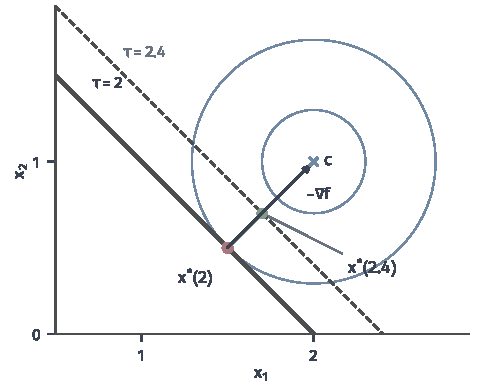
\includegraphics[width=84mm]{figures/05-optimization/06-constrained-optimization/matplotlib/sens-shadow-price-geometry/figure.pdf}
 \caption{预算线平移与乘子。深灰实线是$\tau=2$的预算线，虚线是$\tau=2.4$的预算线，蓝色圆是目标等高线。黑色箭头是$-\nabla f(\bm{x}^\star)=\lambda_1^\star(1,1)$，从红点指向理想点$\bm{c}$。绿色线段是最优解的移动。}
 \label{fig:sens-shadow-price-geometry}
\end{BookInlineFigure}

核对数值。$1<\tau<3$时，$V(\tau)=(3-\tau)^2/4$，这个公式将在第~\ref{sec:sens-active-change}节推出。于是$V'(2)=-1/2=-\lambda_1^\star$。取$\Delta\tau=0.4$，一阶估计是$0.25-0.2=0.05$，真实值$V(2.4)=0.09$。一阶估计恰好等于式~\eqref{eq:sens-budget-bound}的下界，真实值在它上方。

\paragraph{值函数不可微时}
可微性不是自动成立的。下面的引理不要求可微，并且给出了全局下界的完整刻画：所有能作全局下界斜率的向量，恰好就是全体最优乘子的相反数。

\begin{lemma}[下界斜率与最优乘子]
\label{lem:sens-support-multipliers}
设$f^\star$有限，$\bm{\lambda}\in\mathbb{R}^m$，$\bm{\nu}\in\mathbb{R}^p$，$f,g_i,h_j$定义在同一集合$\bm{D}$上，式~\eqref{eq:sens-rhs-value}及对偶函数中的$\bm{x}$都取遍$\bm{D}$。则下面两条等价：
\begin{enumerate}
 \item $\bm{\lambda}\geq\bm{0}$，且$q(\bm{\lambda},\bm{\nu})=f^\star$；
 \item 对所有$(\bm{u},\bm{v})$，都有
 \begin{equation}
  V(\bm{u},\bm{v})\geq f^\star-\langle\bm{\lambda},\bm{u}\rangle-\langle\bm{\nu},\bm{v}\rangle.
  \label{eq:sens-support}
 \end{equation}
\end{enumerate}
\end{lemma}

\begin{proof}
第一条推出第二条，这就是定理~\ref{thm:sens-rhs-bound}。下面从第二条出发。先证明$\lambda_i\geq0$。取$t>0$，令$\bm{u}=t\bm{e}_i$，$\bm{v}=\bm{0}$。放宽约束只会扩大可行集，所以$V(t\bm{e}_i,\bm{0})\leq f^\star$。结合式~\eqref{eq:sens-support}，得到
\[
 f^\star\geq V(t\bm{e}_i,\bm{0})\geq f^\star-t\lambda_i.
\]
所以$\lambda_i\geq0$。

再证明$q(\bm{\lambda},\bm{\nu})\geq f^\star$。任取$\bm{x}\in\bm{D}$，令$u_i=g_i(\bm{x})$，$v_j=h_j(\bm{x})$。这个$\bm{x}$是这组扰动问题的可行点，所以$f(\bm{x})\geq V(\bm{u},\bm{v})$。再由式~\eqref{eq:sens-support}，
\[
 f(\bm{x})\geq f^\star-\sum_i\lambda_ig_i(\bm{x})-\sum_j\nu_jh_j(\bm{x}).
\]

移项得到
\[
 \mathcal{L}(\bm{x},\bm{\lambda},\bm{\nu})\geq f^\star.
\]
对$\bm{x}$取下确界，得到$q(\bm{\lambda},\bm{\nu})\geq f^\star$。又由弱对偶$q(\bm{\lambda},\bm{\nu})\leq f^\star$，所以两者相等。
\end{proof}

当$f$与$g_i$是凸函数、$h_j$是仿射函数时，$V$是凸函数。取两组扰动及各自的近优可行点，它们的凸组合对扰动的相应凸组合仍可行，目标值不超过相应的凸组合，由此就得到$V$的凸性。

这时式~\eqref{eq:sens-support}正是第~\ref{chap:nonsmooth-composite-optimization}章次梯度的定义，引理说的就是$-(\bm{\lambda},\bm{\nu})$属于$V$在原点的次微分。若原点还是$V$的定义域的内点，$V$在方向$(\bm{u},\bm{v})$上的方向导数等于
\begin{equation}
 V'\bigl(\bm{0},\bm{0};\bm{u},\bm{v}\bigr)=\max_{(\bm{\lambda},\bm{\nu})\ \text{最优}}\bigl(-\langle\bm{\lambda},\bm{u}\rangle-\langle\bm{\nu},\bm{v}\rangle\bigr),
 \label{eq:sens-directional}
\end{equation}
其中最大值取遍全部最优乘子。这个等式的证明需要用到凸函数方向导数与次微分的对偶关系，篇幅较长，读者可查阅\scite{rockafellar1970convex}。它的含义是：每个方向上的真实变化率由“最不利”的乘子决定，单独一组乘子不能代表所有方向。

\paragraph{一个有折角的例子}
考虑一维问题
\[
 \min_{x\in\mathbb{R}}\ -x\quad\text{s.t.}\quad x-1\leq u,\ \ x-1\leq0.
\]
两条约束在$u=0$时完全相同，$x^\star=1$，$f^\star=-1$。Lagrange函数是
\[
 \mathcal{L}(x,\bm{\lambda})=(-1+\lambda_1+\lambda_2)x-\lambda_1-\lambda_2.
\]

$\lambda_1+\lambda_2\neq1$时它对$x$无下界。$\lambda_1+\lambda_2=1$时它恒等于$-1$。所以最优乘子集合是线段$\{\bm{\lambda}\geq\bm{0}:\lambda_1+\lambda_2=1\}$，乘子不唯一。

右端扰动的最优值可以直接写出。$u\geq0$时第二条约束决定解，$x=1$；$u<0$时第一条约束决定解，$x=1+u$。所以
\[
 V(u)=\max\{-1-u,\ -1\}.
\]

$V$在$u=0$处有折角，左导数是$-1$，右导数是$0$。图~\ref{fig:sens-subgrad-kink}(a)中斜率在$[-1,0]$内的每条直线都是全局下界，它们恰好对应(b)中线段上的每个乘子。

由式~\eqref{eq:sens-directional}，向右的方向导数$V'(0;1)=\max(-\lambda_1)=0$，由$\lambda_1=0$取到。向左的方向导数$V'(0;-1)=\max\lambda_1=1$，由$\lambda_1=1$取到。求解器如果返回对称的乘子$(1/2,1/2)$，那么$-1/2$只是一个合法的下界斜率，不是任何方向上的导数。

\begin{BookInlineFigure}
 \centering
 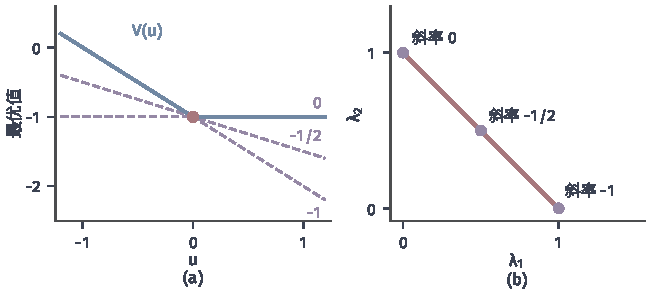
\includegraphics[width=112mm]{figures/05-optimization/06-constrained-optimization/matplotlib/sens-subgrad-kink/figure.pdf}
 \caption{乘子不唯一时的值函数。(a)~蓝线是$V(u)=\max\{-1-u,-1\}$，紫色虚线是斜率$0,-1/2,-1$的全局下界，它们都穿过红点。(b)~红色线段是全体最优乘子，紫色点是图(a)三条直线对应的乘子。}
 \label{fig:sens-subgrad-kink}
\end{BookInlineFigure}

表~\ref{tab:sens-three-slopes}比较本节出现的三个量。

\begin{BookInlineTable}
 \centering
 \begin{tabular}{lll}
  \toprule
  对象 & 成立条件 & 范围\\
  \midrule
  下界斜率$-\bm{\lambda}^\star$ & 零间隙且乘子达到 & 全局，单侧\\
  实际导数$-\bm{\lambda}^\star$ & 另加$V$在基准点可微 & 局部，一阶\\
  方向导数 & 凸问题、基准点在定义域内部 & 局部，沿给定方向\\
  \bottomrule
 \end{tabular}
 \caption{约束右端扰动下的三个量。下界斜率来自任何一组最优乘子，实际导数要求$V$可微，方向导数要在全体最优乘子上取最大值。}
 \label{tab:sens-three-slopes}
\end{BookInlineTable}

\subsection{目标参数的包络关系}
\label{sec:sens-envelope}

现在让目标函数含参数，可行集固定。最优解随参数移动，所以最优值的变化似乎有两个来源：目标本身变了，最优点也动了。本小节的结论是，一阶意义下第二个来源不起作用。

\paragraph{谷底的一阶平坦}
站在谷底，向任何方向走一小步，高度的一阶变化都是零。最优解被参数推着移动一小段，走的正是这样的一小步，所以高度的变化几乎全部来自地形本身的改变。这是整个包络关系的直观基础。

在边界上情况稍有不同：梯度不必为零，因为有约束挡住。但如果解沿着边界来回移动，它向两个相反的方向都是可行的，梯度只能与这个移动方向垂直。

\begin{theorem}[包络关系]
\label{thm:sens-envelope}
设$\bm{C}\subseteq\mathbb{R}^n$固定，$f$在$(\bm{x}_0,\bm{\theta}_0)$的邻域内连续可微。设映射$\bm{x}(\cdot)$定义在$\bm{\theta}_0$的邻域上，取值于$\bm{C}$，在$\bm{\theta}_0$处可微，$\bm{x}(\bm{\theta}_0)=\bm{x}_0$，且$\bm{x}_0$是$f(\cdot,\bm{\theta}_0)$在$\bm{C}$上的局部极小点。记$v$为式~\eqref{eq:sens-branch-value}定义的分支值，则
\begin{equation}
 \nabla v(\bm{\theta}_0)=\nabla_{\bm{\theta}}f(\bm{x}_0,\bm{\theta}_0).
 \label{eq:sens-envelope}
\end{equation}
\end{theorem}

\begin{proof}
记$\bm{D}_{\bm{x}}\in\mathbb{R}^{n\times q}$是$\bm{x}(\cdot)$在$\bm{\theta}_0$的Jacobian矩阵。由链式法则，
\[
 \nabla v(\bm{\theta}_0)=\nabla_{\bm{\theta}}f(\bm{x}_0,\bm{\theta}_0)+\bm{D}_{\bm{x}}^{\top}\nabla_{\bm{x}}f(\bm{x}_0,\bm{\theta}_0).
\]
只需证明第二项为零。任取方向$\bm{d}\in\mathbb{R}^q$，令
\[
 \psi(t)=f\bigl(\bm{x}(\bm{\theta}_0+t\bm{d}),\bm{\theta}_0\bigr).
\]

注意$\psi$里的参数固定在$\bm{\theta}_0$。$\lvert t\rvert$很小时，$\bm{x}(\bm{\theta}_0+t\bm{d})$属于$\bm{C}$且靠近$\bm{x}_0$，所以$\psi(t)\geq\psi(0)$。$t=0$是$\psi$的内部极小点，$\psi'(0)=0$，也就是
\[
 \bigl\langle\nabla_{\bm{x}}f(\bm{x}_0,\bm{\theta}_0),\ \bm{D}_{\bm{x}}\bm{d}\bigr\rangle=0.
\]
$\bm{d}$是任意的，所以
\[
 \bm{D}_{\bm{x}}^{\top}\nabla_{\bm{x}}f(\bm{x}_0,\bm{\theta}_0)=\bm{0}.
\]
\end{proof}

结论说的是分支上的值$v$，而不是全局最优值$V$。条件里最关键的是$\bm{C}$固定：这样分支上的点对基准问题仍是可行的，才能用基准点的局部极小性。约束也含参数的情形放在第~\ref{sec:sens-general-constraints}节。

\paragraph{预算例：理想点移动}
把理想点改成$(2+\theta,1)$，预算固定为$\tau=2$，目标是
\[
 f(\bm{x},\theta)=\frac12(x_1-2-\theta)^2+\frac12(x_2-1)^2.
\]
$\lvert\theta\rvert<1$时只有预算起作用。平稳条件是$x_1-2-\theta+\lambda=0$、$x_2-1+\lambda=0$，与$x_1+x_2=2$联立，得到
\[
 \lambda=\frac{1+\theta}{2},\qquad
 x_1(\theta)=\frac32+\frac{\theta}{2},\qquad
 x_2(\theta)=\frac12-\frac{\theta}{2}.
\]

分支上的值是$v(\theta)=\lambda^2=(1+\theta)^2/4$，直接求导得到$v'(\theta)=(1+\theta)/2$。用包络关系，只需对目标中显含的$\theta$求偏导：
\[
 \frac{\partial f}{\partial\theta}=2+\theta-x_1=\frac{1+\theta}{2}.
\]
两个结果一致。解的移动方向是$\bm{x}'(\theta)=(1/2,-1/2)$，$\nabla_{\bm{x}}f=-\lambda(1,1)$，两者的内积确实为零。图~\ref{fig:sens-envelope}(a)显示，解沿预算线滑动，而负梯度垂直于这条线。

\paragraph{为什么叫包络}
把决策$\hat{\bm{x}}$固定，$\theta\mapsto f(\hat{\bm{x}},\theta)$就是一条曲线。每个固定的决策对应一条这样的曲线，它们都在$v(\theta)$上方，因为固定决策不会比最优决策好。图~\ref{fig:sens-envelope}(b)中$v$是这族曲线的下边缘，称为它们的\emph{包络}，式~\eqref{eq:sens-envelope}因此称为\term{包络定理}（envelope theorem）。

曲线在切点处与$v$相切。切点处的斜率既是这条固定决策曲线的斜率，也是$v$的斜率，这正是“只对显含的$\theta$求导”的图形含义。

\begin{BookInlineFigure}
 \centering
 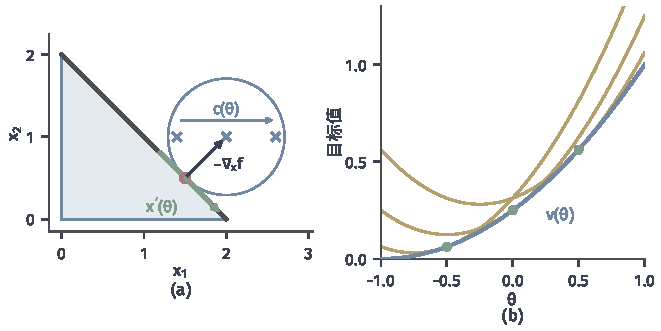
\includegraphics[width=112mm]{figures/05-optimization/06-constrained-optimization/matplotlib/sens-envelope/figure.pdf}
 \caption{包络关系。(a)~$\tau=2$的可行集上，理想点沿蓝色箭头移动（蓝色叉是$\theta=-0.6,0,0.6$），最优解沿绿色线段滑动。红点是$\theta=0$的解，黑色箭头是负梯度，绿色箭头是解的移动方向，两者垂直。(b)~黄线是把决策固定在$\theta=-0.5,0,0.5$的最优解上得到的目标值，蓝线$v(\theta)$是它们的下边缘，绿点是切点。}
 \label{fig:sens-envelope}
\end{BookInlineFigure}

\paragraph{没有可微分支时}
定理~\ref{thm:sens-envelope}需要一条可微的解分支。若最优解不唯一，或最优解随参数跳动，这样的分支就没有了。但只要可行集紧，全局最优值的方向导数仍然有公式，这就是Danskin型结果。

\begin{theorem}[Danskin型结果]
\label{thm:sens-danskin}
设$\bm{C}\subseteq\mathbb{R}^n$非空且紧，$\bm{\Theta}\subseteq\mathbb{R}^q$开，$f$在$\bm{C}\times\bm{\Theta}$上连续，关于$\bm{\theta}$的梯度$\nabla_{\bm{\theta}}f$存在且在$\bm{C}\times\bm{\Theta}$上连续。记$V$为式~\eqref{eq:sens-value}在$\bm{C}(\bm{\theta})\equiv\bm{C}$时的最优值函数，则对每个$\bm{\theta}\in\bm{\Theta}$与方向$\bm{d}$，
\begin{equation}
 V'(\bm{\theta};\bm{d})=\min_{\bm{x}\in\bm{S}(\bm{\theta})}\bigl\langle\nabla_{\bm{\theta}}f(\bm{x},\bm{\theta}),\bm{d}\bigr\rangle.
 \label{eq:sens-danskin}
\end{equation}
若$\bm{S}(\bm{\theta})=\{\bm{x}^\star\}$只有一个点，则$V$在$\bm{\theta}$可微，且
\begin{equation}
 \nabla V(\bm{\theta})=\nabla_{\bm{\theta}}f(\bm{x}^\star,\bm{\theta}).
 \label{eq:sens-danskin-gradient}
\end{equation}
\end{theorem}

\begin{proof}
$\bm{S}(\bm{\theta})$是紧集$\bm{C}$的闭子集，所以式~\eqref{eq:sens-danskin}的最小值可以取到。下面从两个方向夹逼。

先证上界。任取$\bm{x}\in\bm{S}(\bm{\theta})$和$t>0$。$\bm{x}$对$\bm{\theta}+t\bm{d}$仍可行，而且在$\bm{\theta}$处最优，所以
\[
 V(\bm{\theta}+t\bm{d})\leq f(\bm{x},\bm{\theta}+t\bm{d}),\qquad V(\bm{\theta})=f(\bm{x},\bm{\theta}).
\]
由一元中值定理，存在$\xi\in(0,1)$，使
\[
 \frac{V(\bm{\theta}+t\bm{d})-V(\bm{\theta})}{t}\leq\bigl\langle\nabla_{\bm{\theta}}f(\bm{x},\bm{\theta}+\xi t\bm{d}),\bm{d}\bigr\rangle.
\]
令$t\downarrow0$，由梯度的连续性，上极限不超过$\langle\nabla_{\bm{\theta}}f(\bm{x},\bm{\theta}),\bm{d}\rangle$。再对$\bm{x}\in\bm{S}(\bm{\theta})$取最小，就得到上界。

再证下界。取$t_k\downarrow0$，使差商趋于它的下极限，并取$\bm{x}_k\in\bm{S}(\bm{\theta}+t_k\bm{d})$。$\bm{C}$是紧集，可以取子列使$\bm{x}_k\to\bar{\bm{x}}\in\bm{C}$。对任意$\bm{y}\in\bm{C}$，$\bm{x}_k$的最优性给出
\[
 f(\bm{x}_k,\bm{\theta}+t_k\bm{d})\leq f(\bm{y},\bm{\theta}+t_k\bm{d}).
\]
令$k\to\infty$并用$f$的连续性，可知$\bar{\bm{x}}$在参数$\bm{\theta}$下的目标值不超过任何$\bm{y}\in\bm{C}$的目标值，所以$\bar{\bm{x}}\in\bm{S}(\bm{\theta})$。

此外，$\bm{x}_k$是基准问题的可行点，又在$\bm{\theta}+t_k\bm{d}$处最优，所以
\[
 V(\bm{\theta})\leq f(\bm{x}_k,\bm{\theta}),\qquad V(\bm{\theta}+t_k\bm{d})=f(\bm{x}_k,\bm{\theta}+t_k\bm{d}).
\]
再用一次中值定理，存在$\xi_k\in(0,1)$，使
\[
 \frac{V(\bm{\theta}+t_k\bm{d})-V(\bm{\theta})}{t_k}\geq\bigl\langle\nabla_{\bm{\theta}}f(\bm{x}_k,\bm{\theta}+\xi_kt_k\bm{d}),\bm{d}\bigr\rangle.
\]
令$k\to\infty$，下极限不小于$\langle\nabla_{\bm{\theta}}f(\bar{\bm{x}},\bm{\theta}),\bm{d}\rangle$，它又不小于式~\eqref{eq:sens-danskin}的右端。上下界合起来，方向导数存在并等于右端。

只有一个解时，把上面两步中的$t\bm{d}$换成趋于零的向量$\bm{\delta}$。上界一步给出
\[
 V(\bm{\theta}+\bm{\delta})-V(\bm{\theta})\leq\langle\nabla_{\bm{\theta}}f(\bm{x}^\star,\bm{\theta}),\bm{\delta}\rangle+o(\lVert\bm{\delta}\rVert_2).
\]
下界一步中$\bm{x}_{\bm{\delta}}\to\bm{x}^\star$，因为任何极限点都属于单点集$\bm{S}(\bm{\theta})$，于是相同的表达式也是下界。所以$V$可微。
\end{proof}

式~\eqref{eq:sens-danskin}取的是最小值，这与目标是最小化相对应。直观上，参数沿$\bm{d}$变化时，全部最优解处在同一起跑线上，下一时刻仍然留在最优的，是在方向$\bm{d}$上目标增长最慢的那一个。

\paragraph{条件的作用：多解时的方向导数}
考虑线性目标$f(\bm{x},p)=-px_1-x_2$，可行集是$\tau=2$的三角形。$p>1$时最优点是$(2,0)$，$p<1$时最优点是$(0,2)$，$p=1$时整条预算线都是最优解，见图~\ref{fig:sens-danskin-edge}。最优值是
\[
 V(p)=-2\max\{p,1\}.
\]

在$p=1$处，$\partial f/\partial p=-x_1$。式~\eqref{eq:sens-danskin}给出
\[
 V'(1;1)=\min_{\bm{x}\in\bm{S}(1)}(-x_1)=-2,\qquad
 V'(1;-1)=\min_{\bm{x}\in\bm{S}(1)}x_1=0.
\]
第一个由顶点$(2,0)$取到，第二个由顶点$(0,2)$取到，与图中两段的斜率一致。

\begin{BookInlineFigure}
 \centering
 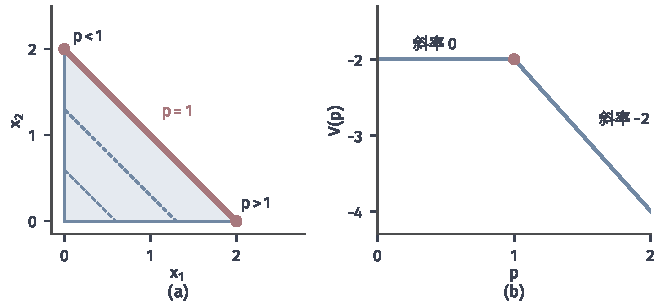
\includegraphics[width=112mm]{figures/05-optimization/06-constrained-optimization/matplotlib/sens-danskin-edge/figure.pdf}
 \caption{线性目标$-px_1-x_2$在三角形$x_1+x_2\leq2$，$\bm{x}\geq\bm{0}$上的最优解。(a)~$p=1$时蓝色虚线的等值线平行于预算线，红色粗线上的点都最优；$p>1$或$p<1$时解是相应的红色顶点。(b)~最优值$V(p)=-2\max\{p,1\}$在$p=1$有折角。}
 \label{fig:sens-danskin-edge}
\end{BookInlineFigure}

紧性不能随意去掉。第~\ref{sec:sens-problems}节的$f(x,\theta)=e^x-\theta x$在$\theta=0$处没有最优解，式~\eqref{eq:sens-danskin}的右端失去意义。实际上$\theta>0$时$V(\theta)=\theta-\theta\ln\theta$，所以
\[
 \frac{V(\theta)-V(0)}{\theta}=1-\ln\theta\to+\infty\quad(\theta\downarrow0),
\]
$V$在$\theta=0$处的右导数不是有限数。

\subsection{一般含参约束}
\label{sec:sens-general-constraints}

现在目标和约束都含参数。可行集随参数移动，上一小节的证明不能直接用，因为分支上的点对基准问题已经不可行。本小节说明，对沿分支的值求导时，Lagrange函数吸收了约束移动的贡献。

\paragraph{从目标到Lagrange函数}
考虑一族问题
\begin{equation}
 \min_{\bm{x}}\ f(\bm{x},\bm{\theta})\quad
 \text{s.t.}\quad g_i(\bm{x},\bm{\theta})\leq0,\ \ h_j(\bm{x},\bm{\theta})=0,
 \label{eq:sens-general-problem}
\end{equation}
其Lagrange函数$\mathcal{L}(\bm{x},\bm{\lambda},\bm{\nu},\bm{\theta})$也含参数。下面的定理假设已经有一条KKT点分支，并且起作用的约束保持起作用。这条分支从何而来，由第~\ref{sec:sens-solution}节回答。

\begin{theorem}[分支值对参数的导数]
\label{thm:sens-general-branch}
设$f,g_i,h_j$在$(\bm{x}_0,\bm{\theta}_0)$的邻域内连续可微。设映射$\bm{x}(\cdot)$在$\bm{\theta}_0$的邻域上满足$\bm{x}(\bm{\theta}_0)=\bm{x}_0$，在$\bm{\theta}_0$可微，$(\bm{x}_0,\bm{\lambda}_0,\bm{\nu}_0)$在$\bm{\theta}_0$处满足平稳条件，且沿分支恒有
\begin{equation}
 g_i(\bm{x}(\bm{\theta}),\bm{\theta})=0\ \ (\lambda_{0,i}>0),\qquad
 h_j(\bm{x}(\bm{\theta}),\bm{\theta})=0.
 \label{eq:sens-active-held}
\end{equation}
记$v$为式~\eqref{eq:sens-branch-value}定义的分支值，则
\begin{equation}
 \nabla v(\bm{\theta}_0)=\nabla_{\bm{\theta}}\mathcal{L}(\bm{x}_0,\bm{\lambda}_0,\bm{\nu}_0,\bm{\theta}_0).
 \label{eq:sens-general-gradient}
\end{equation}
\end{theorem}

\begin{proof}
下面所有函数都在$(\bm{x}_0,\bm{\theta}_0)$取值，$\bm{D}_{\bm{x}}$是分支的Jacobian矩阵。由链式法则，
\[
 \nabla v=\nabla_{\bm{\theta}}f+\bm{D}_{\bm{x}}^{\top}\nabla_{\bm{x}}f.
\]
用平稳条件替换$\nabla_{\bm{x}}f$，乘子为零的项自动消失：
\[
 \bm{D}_{\bm{x}}^{\top}\nabla_{\bm{x}}f=-\sum_{i}\lambda_{0,i}\bm{D}_{\bm{x}}^{\top}\nabla_{\bm{x}}g_i-\sum_j\nu_{0,j}\bm{D}_{\bm{x}}^{\top}\nabla_{\bm{x}}h_j.
\]

对恒等式$g_i(\bm{x}(\bm{\theta}),\bm{\theta})=0$求导，得到
\[
 \bm{D}_{\bm{x}}^{\top}\nabla_{\bm{x}}g_i+\nabla_{\bm{\theta}}g_i=\bm{0}.
\]
等式约束同样如此。代回上一式，得到
\[
 \bm{D}_{\bm{x}}^{\top}\nabla_{\bm{x}}f=\sum_i\lambda_{0,i}\nabla_{\bm{\theta}}g_i+\sum_j\nu_{0,j}\nabla_{\bm{\theta}}h_j.
\]
加上$\nabla_{\bm{\theta}}f$，右端就是$\nabla_{\bm{\theta}}\mathcal{L}$。
\end{proof}

式~\eqref{eq:sens-general-gradient}包含两部分贡献。$\nabla_{\bm{\theta}}f$是目标本身的变化，$\sum\lambda_i\nabla_{\bm{\theta}}g_i$是约束移动造成的变化，乘子把约束的移动折算成目标的变化。若约束不含参数，第二部分为零，回到包络关系。若$g_1=x_1+x_2-\tau$，则$\partial g_1/\partial\tau=-1$，式~\eqref{eq:sens-general-gradient}给出$v'(\tau)=-\lambda_1$，回到边际解释。

\paragraph{一个目标与约束同时含参的例子}
让参数$\theta$同时影响目标和预算的价格：
\[
 \min_{\bm{x}}\ \frac12(x_1-1-\theta)^2+\frac12(x_2-1)^2
 \quad\text{s.t.}\quad \theta x_1+x_2-2\leq0.
\]
$\theta=1$时它就是$\tau=2$的预算例。$\theta$变大时，第一种投入的单价上涨，预算线绕$(0,2)$转动，理想点也同时右移，见图~\ref{fig:sens-moving-constraint}。

\begin{BookInlineFigure}
 \centering
 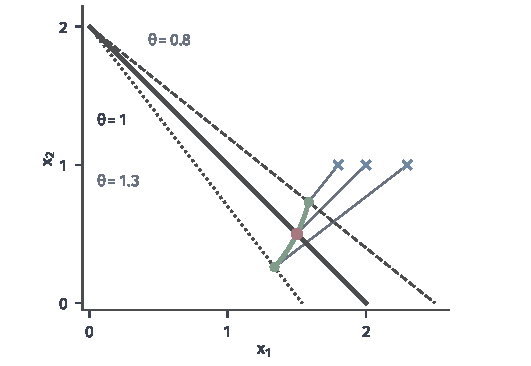
\includegraphics[width=90mm]{figures/05-optimization/06-constrained-optimization/matplotlib/sens-moving-constraint/figure.pdf}
 \caption{目标与约束同时含参。三条深灰线是$\theta=0.8,1,1.3$的预算线$\theta x_1+x_2=2$，蓝色叉是相应的理想点$(1+\theta,1)$，细灰线连接理想点和最优解。绿色曲线是最优解随$\theta$的路径，红点是$\theta=1$的解。}
 \label{fig:sens-moving-constraint}
\end{BookInlineFigure}

预算约束起作用时，平稳条件是$x_1-1-\theta+\lambda\theta=0$、$x_2-1+\lambda=0$。把$x_1=1+\theta-\lambda\theta$与$x_2=1-\lambda$代入$\theta x_1+x_2=2$，解出
\[
 \lambda(\theta)=\frac{\theta^2+\theta-1}{1+\theta^2}.
\]
$\theta=1$时$\lambda=1/2$，$\bm{x}=(3/2,1/2)$。

用式~\eqref{eq:sens-general-gradient}，目标与约束的偏导数分别是
\[
 \frac{\partial f}{\partial\theta}=-(x_1-1-\theta)=\lambda\theta=\frac12,
 \qquad
 \lambda\frac{\partial g}{\partial\theta}=\lambda x_1=\frac34.
\]
相加得到$v'(1)=5/4$。目标的直接变化贡献$1/2$，价格上涨使约束收紧，贡献$3/4$。

直接核对：把解代入目标，得到$v(\theta)=\tfrac12\lambda^2(1+\theta^2)$，即
\[
 v(\theta)=\frac{(\theta^2+\theta-1)^2}{2(1+\theta^2)}.
\]
在$\theta=1$处求导，分子$N=\theta^2+\theta-1$满足$N=1$，$N'=3$，分母$D=1+\theta^2$满足$D=2$，$D'=2$，所以
\[
 v'(1)=\frac{NN'}{D}-\frac{N^2D'}{2D^2}=\frac32-\frac14=\frac54.
\]
两个结果一致。式~\eqref{eq:sens-general-gradient}不需要先解出分支，只需要基准点的$\bm{x}$和乘子。

\section{最优解的变化}
\label{sec:sens-solution}

最优值是一个数，最优解是一个向量，后者需要更多的结构才能求导。这就需要回答：选定一个解之后，它随参数怎样移动？办法是把这个解满足的最优性条件看成一组方程，方程里既有原变量和乘子，也有参数，然后像解隐函数那样求局部导数。

\paragraph{隐函数定理的回顾}
所用的工具是隐函数定理：设$\bm{F}(\bm{z},\bm{\theta})$连续可微，$\bm{F}(\bm{z}_0,\bm{\theta}_0)=\bm{0}$，方阵$\bm{D}_{\bm{z}}\bm{F}(\bm{z}_0,\bm{\theta}_0)$可逆。则在$\bm{\theta}_0$附近有唯一的连续可微映射$\bm{z}(\bm{\theta})$，使$\bm{z}(\bm{\theta}_0)=\bm{z}_0$，且在$(\bm{z}_0,\bm{\theta}_0)$的某个邻域内方程的解全部落在这条曲线上。它的导数满足线性方程
\[
 \bm{D}_{\bm{z}}\bm{F}\cdot\bm{D}\bm{z}=-\bm{D}_{\bm{\theta}}\bm{F}.
\]
定理的陈述与证明可参考\BookChapterRef{chap:implicit-inverse-functions}{卷二第22章“隐函数与反函数”}。

用它研究极小点时要多一步检查，因为隐函数定理只管方程。例如$f(x,\theta)=-x^2/2+\theta x$的驻点方程是$-x+\theta=0$，导数$-1$可逆，隐函数定理给出光滑分支$x(\theta)=\theta$，而这条分支上全是极大点。所以下面每个定理都分成两部分：方程有光滑解，以及这个解确实是极小点。

\subsection{无约束极小解}
\label{sec:sens-unconstrained}

\paragraph{碗的曲率决定碗底移动的距离}
无约束时，$\bm{x}^\star$是碗底，满足$\nabla_{\bm{x}}f=\bm{0}$。参数一变，梯度在原来的位置上不再为零，碗底要移动到新的梯度零点。线性近似告诉我们移动多少：
\[
 \nabla^2_{\bm{x}\bm{x}}f\cdot\Delta\bm{x}+\nabla^2_{\bm{x}\bm{\theta}}f\cdot\Delta\bm{\theta}\approx\bm{0}.
\]
曲率大的方向，碗壁陡，碗底只需移动一点就能抵消参数带来的梯度变化；曲率小的方向，碗底要移动很远。

\begin{theorem}[无约束极小解的导数]
\label{thm:sens-unconstrained}
设$f$在$(\bm{x}_0,\bm{\theta}_0)$的邻域内二阶连续可微，$\nabla_{\bm{x}}f(\bm{x}_0,\bm{\theta}_0)=\bm{0}$，$\nabla^2_{\bm{x}\bm{x}}f(\bm{x}_0,\bm{\theta}_0)\succ\bm{0}$。则存在$\bm{\theta}_0$的邻域和唯一的连续可微映射$\bm{x}(\cdot)$，使$\bm{x}(\bm{\theta}_0)=\bm{x}_0$，且邻域内的每个$\bm{x}(\bm{\theta})$都是$f(\cdot,\bm{\theta})$的严格局部极小点。Jacobian矩阵$\bm{D}_{\bm{x}}\in\mathbb{R}^{n\times q}$由线性方程
\begin{equation}
 \nabla^2_{\bm{x}\bm{x}}f\cdot\bm{D}_{\bm{x}}=-\nabla^2_{\bm{x}\bm{\theta}}f
 \label{eq:sens-unconstrained-derivative}
\end{equation}
确定，其中各导数都在$(\bm{x}(\bm{\theta}),\bm{\theta})$处取值。
\end{theorem}

\begin{proof}
令$\bm{F}=\nabla_{\bm{x}}f$。$f$二阶连续可微，所以$\bm{F}$连续可微。$\bm{D}_{\bm{x}}\bm{F}=\nabla^2_{\bm{x}\bm{x}}f$在基准点正定，因而可逆。隐函数定理给出连续可微的分支$\bm{x}(\bm{\theta})$，对恒等式$\bm{F}(\bm{x}(\bm{\theta}),\bm{\theta})=\bm{0}$求导就得到式~\eqref{eq:sens-unconstrained-derivative}。

再说明它是极小点。Hessian矩阵连续依赖于$(\bm{x},\bm{\theta})$，矩阵的最小特征值连续，所以$\bm{\theta}$靠近$\bm{\theta}_0$时，$\nabla^2_{\bm{x}\bm{x}}f(\bm{x}(\bm{\theta}),\bm{\theta})$仍然正定。驻点处Hessian正定，由第~\ref{chap:smooth-foundations}章的二阶充分条件，$\bm{x}(\bm{\theta})$是严格局部极小点。
\end{proof}

定理是局部的，Hessian正定只说明这条分支是局部极小，它不保证全局最优。正定性也不能减弱成可逆：上面驻点是极大点的例子中，Hessian可逆但负定。

\paragraph{例子：带二次惩罚的最小二乘}
取$\bm{A}$和$\bm{b}$如下，并用$\gamma>0$作正则系数：
\[
 \bm{A}=\begin{bmatrix}1&1\\1&0\end{bmatrix},\qquad
 \bm{b}=\begin{bmatrix}2\\0\end{bmatrix},\qquad
 f(\bm{x},\gamma)=\frac12\lVert\bm{A}\bm{x}-\bm{b}\rVert_2^2+\frac{\gamma}{2}\lVert\bm{x}\rVert_2^2.
\]
梯度为零的方程是$\bm{H}(\gamma)\bm{x}=\bm{A}^{\top}\bm{b}$，其中
\[
 \bm{H}(\gamma)=\bm{A}^{\top}\bm{A}+\gamma\bm{I}=\begin{bmatrix}2+\gamma&1\\1&1+\gamma\end{bmatrix},\qquad
 \bm{A}^{\top}\bm{b}=\begin{bmatrix}2\\2\end{bmatrix}.
\]

$\gamma>0$时$\bm{H}(\gamma)$正定，所以全局最优解存在且唯一，条件满足。在$\gamma=1$处，求$\bm{H}$的逆矩阵，得到
\[
 \bm{H}(1)=\begin{bmatrix}3&1\\1&2\end{bmatrix},\qquad
 \bm{H}(1)^{-1}=\frac15\begin{bmatrix}2&-1\\-1&3\end{bmatrix},\qquad
 \bm{x}(1)=\begin{bmatrix}2/5\\4/5\end{bmatrix}.
\]

梯度$\bm{H}(\gamma)\bm{x}-\bm{A}^{\top}\bm{b}$对$\gamma$的偏导数是$\bm{x}$本身。于是式~\eqref{eq:sens-unconstrained-derivative}给出
\[
 \bm{x}'(1)=-\bm{H}(1)^{-1}\bm{x}(1)=\begin{bmatrix}0\\-2/5\end{bmatrix}.
\]

$\gamma$增大时，解在这一点上只往$x_2$减小的方向移动，$x_1$的一阶变化恰好为零。显式解是
\[
 x_1(\gamma)=\frac{2\gamma}{1+3\gamma+\gamma^2},\qquad
 x_2(\gamma)=\frac{2+2\gamma}{1+3\gamma+\gamma^2},
\]
直接求导可以验证同一结果，$x_1(\gamma)$恰在$\gamma=1$达到最大。

\paragraph{局部导数与有限跳变}
一阶预测$\bm{x}(1)+(\gamma-1)\bm{x}'(1)$的可信范围是有限的。$\gamma=1.1$时，真解和预测分别是
\[
 \bm{x}(1.1)\approx(0.3993,\ 0.7623),\qquad
 \bm{x}(1)+0.1\,\bm{x}'(1)=(0.4,\ 0.76).
\]
两者很接近。$\gamma=3$时，真解是$(6/19,8/19)\approx(0.316,0.421)$，而预测是$(0.4,0)$，差得很远。图~\ref{fig:sens-ridge-path}显示了原因：解的路径是弯的，切线只在基准点附近贴着它。

\begin{BookInlineFigure}
 \centering
 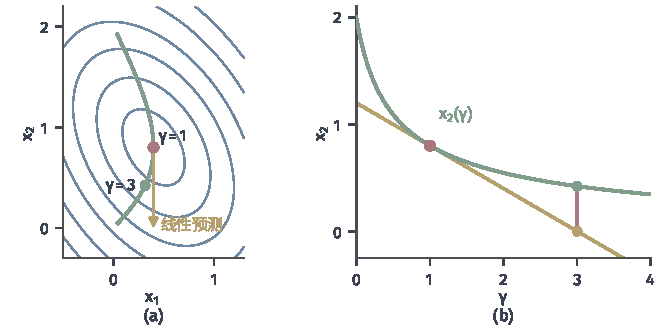
\includegraphics[width=112mm]{figures/05-optimization/06-constrained-optimization/matplotlib/sens-ridge-path/figure.pdf}
 \caption{带二次惩罚的最小二乘的解随$\gamma$的移动。(a)~蓝线是$\gamma=1$的目标等高线，绿色曲线是解的路径，红点是$\bm{x}(1)$，绿点是$\bm{x}(3)$，黄色箭头是导数给出的线性预测。(b)~$x_2(\gamma)$（绿线）与它在$\gamma=1$的切线（黄线），红色线段是$\gamma=3$处的预测误差。}
 \label{fig:sens-ridge-path}
\end{BookInlineFigure}

导数回答的是无穷小的变化。有限跳变需要另外的工具。下面的结论不需要解分支可微，对任意大小的参数差都成立。

\begin{theorem}[强凸情形的有限跳变界]
\label{thm:sens-finite-jump}
设对$\bm{\theta}\in\{\bm{\theta}_0,\bm{\theta}_1\}$，$f(\cdot,\bm{\theta})$在$\mathbb{R}^n$上可微，$\bm{x}_0$、$\bm{x}_1$分别是$f(\cdot,\bm{\theta}_0)$、$f(\cdot,\bm{\theta}_1)$的最小点，且$f(\cdot,\bm{\theta}_1)$是$\mu$强凸的。则
\begin{equation}
 \lVert\bm{x}_1-\bm{x}_0\rVert_2\leq\frac{1}{\mu}\bigl\lVert\nabla_{\bm{x}}f(\bm{x}_0,\bm{\theta}_1)-\nabla_{\bm{x}}f(\bm{x}_0,\bm{\theta}_0)\bigr\rVert_2.
 \label{eq:sens-finite-jump}
\end{equation}
\end{theorem}

\begin{proof}
强凸函数的梯度满足
\[
 \bigl\langle\nabla_{\bm{x}}f(\bm{x}_1,\bm{\theta}_1)-\nabla_{\bm{x}}f(\bm{x}_0,\bm{\theta}_1),\ \bm{x}_1-\bm{x}_0\bigr\rangle\geq\mu\lVert\bm{x}_1-\bm{x}_0\rVert_2^2.
\]
$\bm{x}_1$是$f(\cdot,\bm{\theta}_1)$的最小点，所以左端第一个梯度为零。$\bm{x}_0$是基准问题的最小点，零向量$\nabla_{\bm{x}}f(\bm{x}_0,\bm{\theta}_0)$可以加进去而不改变左端。于是
\[
 \mu\lVert\bm{x}_1-\bm{x}_0\rVert_2^2\leq\bigl\langle\nabla_{\bm{x}}f(\bm{x}_0,\bm{\theta}_0)-\nabla_{\bm{x}}f(\bm{x}_0,\bm{\theta}_1),\ \bm{x}_1-\bm{x}_0\bigr\rangle.
\]
用Cauchy--Schwarz不等式放大右端，再除以$\lVert\bm{x}_1-\bm{x}_0\rVert_2$（为零时结论直接成立），就得到式~\eqref{eq:sens-finite-jump}。
\end{proof}

式~\eqref{eq:sens-finite-jump}右端衡量“新目标在旧解处的梯度有多大”，$1/\mu$把这个梯度折算成距离，这与隐式导数中的逆Hessian起同样的作用。

在岭回归的例子里，$\gamma_0=1$，$\gamma_1=3$，新旧目标在$\bm{x}_0$处的梯度差是$(\gamma_1-\gamma_0)\bm{x}_0$，强凸常数是
\[
 \mu=3+\lambda_{\min}(\bm{A}^{\top}\bm{A})=3+\frac{3-\sqrt{5}}{2}.
\]
算出的上界和真实距离分别是
\[
 \frac{2\lVert\bm{x}_0\rVert_2}{\mu}\approx0.529,\qquad
 \lVert\bm{x}(3)-\bm{x}(1)\rVert_2\approx0.388.
\]
真实距离没有超过上界。

\paragraph{预测误差受三阶信息控制}
一阶预测的误差要看导数变化得多快。下面的情形最容易说清楚：参数以线性项进入目标。

\begin{theorem}[线性扰动下的预测误差]
\label{thm:sens-prediction-error}
设$\varphi:\mathbb{R}^n\to\mathbb{R}$二阶连续可微、$\mu$强凸，$\nabla^2\varphi$是$M$-Lipschitz连续的。令
\begin{equation}
 f(\bm{x},\bm{\theta})=\varphi(\bm{x})-\langle\bm{\theta},\bm{x}\rangle,
 \label{eq:sens-linear-perturbation}
\end{equation}
$\bm{x}(\bm{\theta})$是唯一最小点，$\bm{H}=\nabla^2\varphi(\bm{x}(\bm{\theta}))$。则对任意$\bm{\Delta}\in\mathbb{R}^n$，
\begin{equation}
 \bigl\lVert\bm{x}(\bm{\theta}+\bm{\Delta})-\bm{x}(\bm{\theta})-\bm{H}^{-1}\bm{\Delta}\bigr\rVert_2\leq\frac{M}{2\mu^3}\lVert\bm{\Delta}\rVert_2^2.
 \label{eq:sens-prediction-error}
\end{equation}
\end{theorem}

\begin{proof}
记$\bm{x}=\bm{x}(\bm{\theta})$，$\bm{p}=\bm{x}(\bm{\theta}+\bm{\Delta})-\bm{x}$。两点的驻点方程相减，得到
\[
 \nabla\varphi(\bm{x}+\bm{p})-\nabla\varphi(\bm{x})=\bm{\Delta}.
\]
把左端写成Hessian矩阵的积分，再用Lipschitz条件，得到
\[
 \bigl\lVert\nabla\varphi(\bm{x}+\bm{p})-\nabla\varphi(\bm{x})-\bm{H}\bm{p}\bigr\rVert_2\leq\frac{M}{2}\lVert\bm{p}\rVert_2^2,
\]
也就是
\[
 \lVert\bm{\Delta}-\bm{H}\bm{p}\rVert_2\leq\frac{M}{2}\lVert\bm{p}\rVert_2^2.
\]

$\bm{H}$的最小特征值不小于$\mu$，所以两边乘以$\bm{H}^{-1}$后，
\[
 \lVert\bm{H}^{-1}\bm{\Delta}-\bm{p}\rVert_2\leq\frac{M}{2\mu}\lVert\bm{p}\rVert_2^2.
\]
再用定理~\ref{thm:sens-finite-jump}。这里梯度差的范数恰好是$\lVert\bm{\Delta}\rVert_2$，所以
\[
 \lVert\bm{p}\rVert_2\leq\frac{1}{\mu}\lVert\bm{\Delta}\rVert_2.
\]
代入上式，就得到式~\eqref{eq:sens-prediction-error}。
\end{proof}

$M=0$时目标是二次的，预测对任意大小的$\bm{\Delta}$都精确。上面最小二乘例子中，$\bm{b}$的变化正是这种情形：$\bm{x}$是$\bm{b}$的线性函数，一阶预测不会有误差。$\gamma$的变化不属于线性扰动，因为它改变了曲率本身，这正是图~\ref{fig:sens-ridge-path}中路径弯曲的原因。

\subsection{等式约束极小解}
\label{sec:sens-equality}

有等式约束时，极小点不再是梯度的零点，而是Lagrange函数的驻点，方程组里要把乘子一并算上。本小节要说明，所需的正定性只需在约束的切空间上成立。

\paragraph{联合方程}
考虑
\[
 \min_{\bm{x}}\ f(\bm{x},\bm{\theta})\quad\text{s.t.}\quad\bm{h}(\bm{x},\bm{\theta})=\bm{0},\qquad\bm{h}:\mathbb{R}^n\times\mathbb{R}^q\to\mathbb{R}^p.
\]
解$\bm{x}$和乘子$\bm{\nu}$同时满足平稳条件和可行条件，共$n+p$个方程，未知量也是$n+p$个：
\begin{equation}
 \bm{F}(\bm{x},\bm{\nu},\bm{\theta})=\begin{bmatrix}\nabla_{\bm{x}}\mathcal{L}(\bm{x},\bm{\nu},\bm{\theta})\\\bm{h}(\bm{x},\bm{\theta})\end{bmatrix}=\bm{0}.
 \label{eq:sens-kkt-equation}
\end{equation}

记$\bm{W}=\nabla^2_{\bm{x}\bm{x}}\mathcal{L}$，$\bm{J}=\bm{D}_{\bm{x}}\bm{h}$（$p\times n$矩阵，第$j$行是$\nabla_{\bm{x}}h_j^{\top}$）。$\bm{F}$关于$(\bm{x},\bm{\nu})$的Jacobian矩阵是
\begin{equation}
 \bm{K}=\begin{bmatrix}\bm{W}&\bm{J}^{\top}\\\bm{J}&\bm{0}\end{bmatrix}.
 \label{eq:sens-kkt-matrix}
\end{equation}
称为\term{KKT矩阵}（KKT matrix）。隐函数定理需要它可逆。下面的引理说明，这正是约束梯度独立和切空间曲率为正共同保证的。

\begin{lemma}[KKT矩阵可逆]
\label{lem:sens-kkt-invertible}
设$\bm{J}\in\mathbb{R}^{r\times n}$行满秩，$\bm{W}\in\mathbb{R}^{n\times n}$对称，并且对每个满足$\bm{J}\bm{d}=\bm{0}$的非零向量$\bm{d}$，都有$\bm{d}^{\top}\bm{W}\bm{d}>0$。则式~\eqref{eq:sens-kkt-matrix}的矩阵$\bm{K}$可逆。
\end{lemma}

\begin{proof}
$\bm{K}$是方阵，只需证明它的零空间只含零向量。设$\bm{K}$作用在$(\bm{d},\bm{w})$上为零，也就是
\[
 \bm{W}\bm{d}+\bm{J}^{\top}\bm{w}=\bm{0},\qquad\bm{J}\bm{d}=\bm{0}.
\]
用$\bm{d}^{\top}$左乘第一式，再用第二式，得到
\[
 \bm{d}^{\top}\bm{W}\bm{d}=-(\bm{J}\bm{d})^{\top}\bm{w}=0.
\]

由切空间上的正定性，$\bm{d}=\bm{0}$。第一式于是成为$\bm{J}^{\top}\bm{w}=\bm{0}$。$\bm{J}$行满秩，所以$\bm{w}=\bm{0}$。
\end{proof}

两个条件的分工很清楚。正定性排除了沿约束方向走而曲率为零的情形，行满秩排除了乘子有多种取法的情形。

\begin{theorem}[等式约束极小解的导数]
\label{thm:sens-equality}
设$f,\bm{h}$在$(\bm{x}_0,\bm{\theta}_0)$的邻域内二阶连续可微，$(\bm{x}_0,\bm{\nu}_0)$在$\bm{\theta}_0$处满足式~\eqref{eq:sens-kkt-equation}，$\bm{J}$行满秩，且$\bm{W}$在$\ker\bm{J}$上正定。则存在$\bm{\theta}_0$的邻域和唯一的连续可微映射$(\bm{x}(\cdot),\bm{\nu}(\cdot))$，满足式~\eqref{eq:sens-kkt-equation}并经过基准点，每个$\bm{x}(\bm{\theta})$都是相应问题的严格局部极小点，乘子唯一。导数满足
\begin{equation}
 \begin{bmatrix}\bm{W}&\bm{J}^{\top}\\\bm{J}&\bm{0}\end{bmatrix}
 \begin{bmatrix}\bm{D}_{\bm{x}}\\\bm{D}_{\bm{\nu}}\end{bmatrix}
 =-\begin{bmatrix}\nabla^2_{\bm{x}\bm{\theta}}\mathcal{L}\\\bm{D}_{\bm{\theta}}\bm{h}\end{bmatrix}.
 \label{eq:sens-equality-derivative}
\end{equation}
\end{theorem}

\begin{proof}
由引理~\ref{lem:sens-kkt-invertible}，$\bm{K}$在基准点可逆。$f,\bm{h}$二阶连续可微，所以$\bm{F}$连续可微，隐函数定理给出分支，对恒等式$\bm{F}=\bm{0}$求导就得到式~\eqref{eq:sens-equality-derivative}。

下面说明两个条件在基准点附近保持。行满秩是开条件，因为某个$p$阶子式不为零，它在附近仍不为零。

对切空间上的正定性用反证法。若有$\bm{\theta}_k\to\bm{\theta}_0$，以及单位向量$\bm{d}_k$，满足$\bm{J}_k\bm{d}_k=\bm{0}$，$\bm{d}_k^{\top}\bm{W}_k\bm{d}_k\leq0$，取收敛子列$\bm{d}_k\to\bm{d}$，则$\bm{J}\bm{d}=\bm{0}$，$\bm{d}^{\top}\bm{W}\bm{d}\leq0$，$\lVert\bm{d}\rVert_2=1$，这与假设矛盾。

于是分支上每一点都满足第~\ref{chap:constrained-optimality}章的二阶充分条件：KKT点处，Lagrange Hessian在约束切空间上正定，保证该点是严格局部极小点。乘子由$\bm{J}^{\top}\bm{\nu}=-\nabla_{\bm{x}}f$和行满秩唯一确定。
\end{proof}

\paragraph{预算线上的例子}
把预算例的预算约束写成等式$x_1+x_2-\tau=0$，$\bm{W}=\bm{I}$，$\bm{J}=(1,1)$，$\partial h/\partial\tau=-1$，$\nabla^2_{\bm{x}\tau}\mathcal{L}=\bm{0}$。式~\eqref{eq:sens-equality-derivative}写成
\[
 \begin{bmatrix}1&0&1\\0&1&1\\1&1&0\end{bmatrix}
 \begin{bmatrix}x_1'\\x_2'\\\nu'\end{bmatrix}
 =\begin{bmatrix}0\\0\\1\end{bmatrix}.
\]
前两行说明$x_1'=x_2'=-\nu'$，第三行给出$2x_1'=1$。于是
\[
 x_1'=x_2'=\frac12,\qquad\nu'=-\frac12.
\]
多一单位预算平均分给两种投入，因为二次损失在两个方向上曲率相同。

\paragraph{整个空间上不必正定}
这个例子的$\bm{W}$碰巧正定，下面的例子不是。在预算线上使乘积最大，等价于
\[
 \min_{\bm{x}}\ -x_1x_2\quad\text{s.t.}\quad h(\bm{x},\theta)=\theta x_1+x_2-2=0,
\]
参数$\theta$是第一种投入的价格。先取基准$\theta=1$。平稳条件是$-x_2+\nu\theta=0$、$-x_1+\nu=0$，与约束联立，得到
\[
 x_1(\theta)=\frac{1}{\theta},\qquad x_2(\theta)=1,\qquad\nu(\theta)=\frac{1}{\theta}.
\]

基准点是$\bm{x}_0=(1,1)$，$\nu_0=1$。$\bm{W}$的特征值是$\pm1$，它不定，而切方向$\bm{d}=(1,-1)$上
\[
 \bm{W}=\begin{bmatrix}0&-1\\-1&0\end{bmatrix},\qquad
 \bm{d}^{\top}\bm{W}\bm{d}=2>0.
\]
图~\ref{fig:sens-equality-tangent}说明了这一点。沿着约束，Lagrange函数向上弯；垂直于约束，它向下弯。但可行点不能离开约束线，所以垂直方向的负曲率不影响极小性。

\begin{BookInlineFigure}
 \centering
 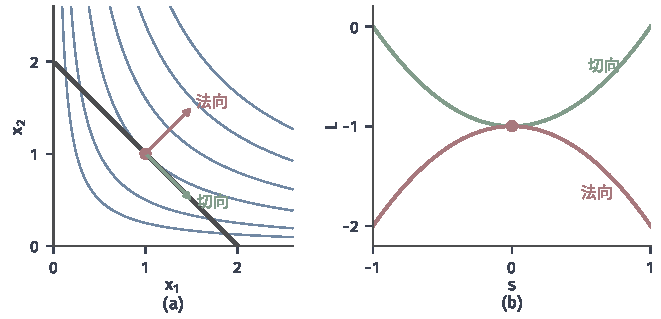
\includegraphics[width=112mm]{figures/05-optimization/06-constrained-optimization/matplotlib/sens-equality-tangent/figure.pdf}
 \caption{切空间上的正定性。(a)~蓝线是$x_1x_2$的等值线，深灰线是约束$x_1+x_2=2$，红点是解，绿色箭头是切方向，红色箭头是法方向。(b)~取$\nu=1$，Lagrange函数沿切方向$(1+s,1-s)$的值是$s^2-1$（绿线），沿法方向$(1+s,1+s)$的值是$-1-s^2$（红线）。}
 \label{fig:sens-equality-tangent}
\end{BookInlineFigure}

Lagrange函数对$\bm{x}$的梯度是
\[
 \nabla_{\bm{x}}\mathcal{L}=(-x_2+\nu\theta,\ -x_1+\nu),
\]
它对$\theta$的偏导数是$(\nu,0)$，而$\partial h/\partial\theta=x_1$。在基准点，这些量都已知，式~\eqref{eq:sens-equality-derivative}成为
\[
 \begin{bmatrix}0&-1&1\\-1&0&1\\1&1&0\end{bmatrix}
 \begin{bmatrix}x_1'\\x_2'\\\nu'\end{bmatrix}
 =-\begin{bmatrix}1\\0\\1\end{bmatrix}.
\]

第二行给出$\nu'=x_1'$，第一行给出$x_2'=x_1'+1$，代入第三行$x_1'+x_2'=-1$，得到
\[
 x_1'=-1,\qquad x_2'=0,\qquad\nu'=-1.
\]
这与显式解在$\theta=1$的导数一致：涨价时第一种投入减少，第二种投入不变。

如果把目标改成$+x_1x_2$，KKT矩阵仍然可逆，隐函数定理仍然给出同样的分支，但切方向的曲率变成$-2$，这条分支上全是约束极大点。可逆只说明方程的解光滑，极小性要靠曲率的符号。

\paragraph{去掉条件会怎样}
先去掉切空间正定性。考虑$\min\tfrac12x_2^2$，约束$x_2-\theta=0$。约束梯度$(0,1)$非零，但切方向$(1,0)$上$\bm{W}=\operatorname{diag}(0,1)$的曲率为零。此时$\bm{K}$的第一行全为零，矩阵奇异。解集是整条直线$\{(s,\theta):s\in\mathbb{R}\}$，“解的导数”没有确定的含义。

再去掉行满秩。考虑$\min x$，约束$x^2-\theta=0$。$\theta>0$时可行集是$\{\pm\sqrt{\theta}\}$，最小点是$x=-\sqrt{\theta}$，导数是$-1/(2\sqrt{\theta})$，$\theta\downarrow0$时趋于$-\infty$。在$\theta=0$处约束梯度$2x$为零，平稳条件$1+2x\nu=0$在$x=0$处没有解，KKT条件本身就不成立。

\subsection{不等式约束极小解}
\label{sec:sens-inequality}

不等式比等式多了一件事：哪些约束起作用，可能随参数改变。本小节的思路是，只要局部上活动约束不变，就把它们当作等式，回到上一小节的情形。

\paragraph{需要的三个条件}
考虑一般问题~\eqref{eq:sens-general-problem}，设$(\bm{x}_0,\bm{\lambda}_0,\bm{\nu}_0)$是$\bm{\theta}_0$处的KKT点，$A=\{i:g_i(\bm{x}_0,\bm{\theta}_0)=0\}$是活动集，$a$是其元素个数。这里用到第~\ref{chap:constrained-optimality}章的三个概念。

\begin{itemize}
 \item \emph{线性无关约束资格}（LICQ）：活动不等式的梯度和全部等式的梯度线性无关。
 \item \emph{严格互补}：每个活动不等式的乘子都严格为正，$\lambda_{0,i}>0$（$i\in A$）。
 \item \emph{二阶充分条件}：$\bm{W}=\nabla^2_{\bm{x}\bm{x}}\mathcal{L}$在临界锥上正定。严格互补成立时，临界锥就是子空间$\ker\bm{J}$，其中$\bm{J}$的行是活动不等式和全部等式的梯度。
\end{itemize}

把活动的不等式改写成等式，定义未知向量$\bm{w}=(\bm{\lambda}_A,\bm{\nu})$，得到一个缩减的方程组
\begin{equation}
 \bm{F}(\bm{x},\bm{w},\bm{\theta})=\begin{bmatrix}\nabla_{\bm{x}}\mathcal{L}\\\bm{g}_A(\bm{x},\bm{\theta})\\\bm{h}(\bm{x},\bm{\theta})\end{bmatrix}=\bm{0}.
 \label{eq:sens-reduced-kkt}
\end{equation}
活动约束的乘子和等式乘子是未知量，不活动约束的乘子取为零，不进入方程。

\begin{theorem}[不等式约束极小解的导数]
\label{thm:sens-inequality}
设$f,g_i,h_j$在$(\bm{x}_0,\bm{\theta}_0)$的邻域内二阶连续可微，$(\bm{x}_0,\bm{\lambda}_0,\bm{\nu}_0)$是KKT点，LICQ、严格互补与二阶充分条件成立。则存在$\bm{\theta}_0$的邻域和唯一的连续可微映射$(\bm{x}(\cdot),\bm{\lambda}(\cdot),\bm{\nu}(\cdot))$，它在基准处经过基准点，邻域内的每一点都是相应问题的KKT点，活动集恒为$A$，$\bm{x}(\bm{\theta})$是严格局部极小点。导数$\bm{D}_{\bm{x}}$、$\bm{D}_{\bm{w}}$满足
\begin{equation}
 \begin{bmatrix}\bm{W}&\bm{J}^{\top}\\\bm{J}&\bm{0}\end{bmatrix}
 \begin{bmatrix}\bm{D}_{\bm{x}}\\\bm{D}_{\bm{w}}\end{bmatrix}
 =-\begin{bmatrix}\nabla^2_{\bm{x}\bm{\theta}}\mathcal{L}\\\bm{D}_{\bm{\theta}}(\bm{g}_A,\bm{h})\end{bmatrix}.
 \label{eq:sens-inequality-derivative}
\end{equation}
\end{theorem}

\begin{proof}
LICQ就是$\bm{J}$行满秩，严格互补使二阶充分条件成为$\bm{W}$在$\ker\bm{J}$上正定。由引理~\ref{lem:sens-kkt-invertible}，矩阵$\bm{K}$可逆，隐函数定理给出式~\eqref{eq:sens-reduced-kkt}的连续可微解$(\bm{x}(\bm{\theta}),\bm{w}(\bm{\theta}))$，求导得到式~\eqref{eq:sens-inequality-derivative}。

下面验证这个解确实是完整问题的KKT点。不活动约束满足$g_i(\bm{x}_0,\bm{\theta}_0)<0$，由连续性，附近仍有$g_i(\bm{x}(\bm{\theta}),\bm{\theta})<0$，把它们的乘子取为零。活动约束的乘子满足$\lambda_{0,i}>0$，由连续性，附近仍有$\lambda_i(\bm{\theta})>0$。于是可行性、乘子符号和互补松弛全部成立，活动集仍是$A$，且严格互补仍成立。

与定理~\ref{thm:sens-equality}相同的连续性论证说明，$\bm{J}$行满秩和$\ker\bm{J}$上的正定性在附近保持，二阶充分条件推出$\bm{x}(\bm{\theta})$是严格局部极小点。

最后看唯一性。若完整问题另有KKT点靠近基准点，不活动约束仍严格满足，其乘子必为零；活动约束的乘子靠近正数$\lambda_{0,i}$，也为正，由互补松弛这些约束取等号。这个点于是满足式~\eqref{eq:sens-reduced-kkt}，由隐函数定理的唯一性，它就在分支上。
\end{proof}

图~\ref{fig:sens-kkt-block}画出式~\eqref{eq:sens-inequality-derivative}的结构。系数矩阵只由基准点的量决定，$q$个参数对应$q$列右端。

\begin{BookInlineFigure}
 \centering
 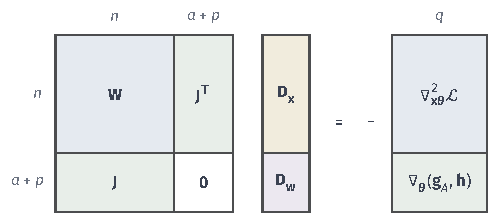
\includegraphics[width=83mm]{figures/05-optimization/06-constrained-optimization/tikz/sens-kkt-block/figure.pdf}
 \caption{式~\eqref{eq:sens-inequality-derivative}的分块结构。系数矩阵的阶数是$n+a+p$，其中$a$是活动不等式个数，$p$是等式个数。$\bm{D}_{\bm{x}}$与$\bm{D}_{\bm{w}}$是待求的Jacobian矩阵，右端共$q$列，每列对应一个参数。不活动约束不出现在这个方程组中。}
 \label{fig:sens-kkt-block}
\end{BookInlineFigure}

\paragraph{预算例的两个活动集}
取$\tau=2$。活动集是$\{1\}$，方程组与第~\ref{sec:sens-equality}节的预算线例子完全相同，因为只有预算在起作用：
\[
 x_1'=x_2'=\frac12,\qquad\lambda_1'=-\frac12.
\]

取$\tau=0.5$。解是$(0.5,0)$，乘子是$\lambda_1=3/2$，$\lambda_3=1/2$，活动集是$\{1,3\}$。此时$\bm{W}=\bm{I}$，活动约束的梯度组成
\[
 \bm{J}=\begin{bmatrix}1&1\\0&-1\end{bmatrix},\qquad
 \frac{\partial}{\partial\tau}\begin{bmatrix}g_1\\g_3\end{bmatrix}=\begin{bmatrix}-1\\0\end{bmatrix}.
\]

$\ker\bm{J}$只含零向量，切空间的正定性自动成立。式~\eqref{eq:sens-inequality-derivative}的四行分别是
\[
 x_1'+\lambda_1'=0,\quad
 x_2'+\lambda_1'-\lambda_3'=0,\quad
 x_1'+x_2'=1,\quad
 -x_2'=0.
\]
依次解出
\[
 x_2'=0,\qquad x_1'=1,\qquad\lambda_1'=-1,\qquad\lambda_3'=-1.
\]
这时增加的预算全部给第一种投入，因为$x_2$被边界挡在零上。

\paragraph{严格互补和余量给出窗口}
严格互补与不活动约束的严格余量在定理中起同一种作用：它们留出一段余地，让参数小幅变化时符号条件不被破坏。这段余地有多大，可以用导数估计。

在$\tau=2$处，三个要保持为正的量分别是不活动约束的余量$x_1$、$x_2$和活动约束的乘子$\lambda_1$。沿分支它们是
\[
 x_1=\frac{\tau+1}{2},\qquad
 x_2=\frac{\tau-1}{2},\qquad
 \lambda_1=\frac{3-\tau}{2}.
\]

第一个到达零的是$x_2$（$\tau=1$）和$\lambda_1$（$\tau=3$），分支的有效窗口是$1<\tau<3$，见图~\ref{fig:sens-margins}。窗口的一端是不活动约束变成活动，另一端是活动约束不再起作用。

\begin{BookInlineFigure}
 \centering
 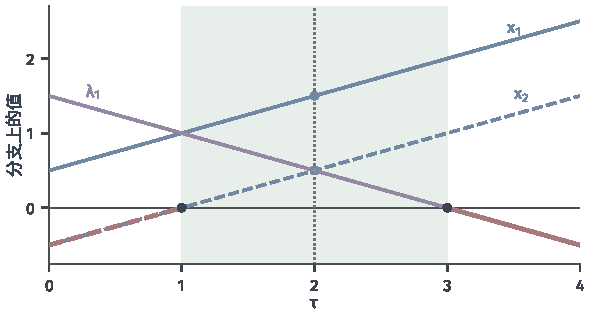
\includegraphics[width=100mm]{figures/05-optimization/06-constrained-optimization/matplotlib/sens-margins/figure.pdf}
 \caption{活动集$\{1\}$的分支把公式延拓到窗口之外。蓝色实线与虚线是不活动约束的余量$x_1$、$x_2$，紫线是乘子$\lambda_1$，绿色区域是三者都为正的窗口$1<\tau<3$。红色部分是符号条件被破坏之处：$\tau<1$时$x_2<0$不可行，$\tau>3$时$\lambda_1<0$不满足KKT条件。}
 \label{fig:sens-margins}
\end{BookInlineFigure}

\paragraph{这些条件只是充分的}
定理的三个条件对解可微是充分条件，下面三个例子逐一说明它们都不是必要的。

严格互补不必要：考虑$\min\tfrac12(x-\theta^2)^2$，约束$x\geq0$。解是$x=\theta^2$，处处可微。而在$\theta=0$处，约束活动且乘子为零，严格互补不成立。

LICQ不必要：约束写两遍$\theta-x\leq0$，目标取$\min x$。解$x=\theta$处处可微，两条活动约束的梯度相同，LICQ不成立，乘子也不唯一。

二阶充分条件不必要：考虑$\min x^4/4-\theta^3x$，驻点方程$x^3=\theta^3$给出$x=\theta$，处处可微。而在$\theta=0$处Hessian等于零。

反过来，这些条件被破坏时，导数常常确实失效，下一节拆开具体的失效方式。定理不能用来断言“条件不成立，所以不可微”。

\section{分支变化}
\label{sec:sens-branches}

上一节的局部导数有前提。前提不成立时，导数为什么会失效，失效的方式有什么不同？本节用三个能够手算的例子回答。活动集改变时，可用的方程变了。全局最优解切换时，所选的分支变了。方程退化时，线性方程不再可逆。三种情况的数学原因不同，都不是某个算法的不稳定。

\subsection{活动集改变}
\label{sec:sens-active-change}

\paragraph{分段解出预算例}
把预算例按活动集分成三段，每段都用KKT条件解出。

当$\tau>3$时，理想点$(2,1)$满足$x_1+x_2\leq\tau$，全部约束不起作用：
\[
 \bm{x}^\star=(2,1),\qquad\bm{\lambda}=\bm{0},\qquad V(\tau)=0.
\]

当$1<\tau<3$时，只有预算起作用。平稳条件是$x_1-2+\lambda_1=0$、$x_2-1+\lambda_1=0$，代入$x_1+x_2=\tau$，得到$3-2\lambda_1=\tau$，于是
\[
 \lambda_1=\frac{3-\tau}{2},\qquad
 \bm{x}^\star=\Bigl(\frac{\tau+1}{2},\ \frac{\tau-1}{2}\Bigr).
\]
两个坐标与乘子在这段都是正的。目标值是$\lambda_1^2$，即$V(\tau)=(3-\tau)^2/4$。

当$0<\tau<1$时，预算和$x_2\geq0$起作用，$\bm{x}^\star=(\tau,0)$。平稳条件的两个分量是$x_1-2+\lambda_1=0$和$x_2-1+\lambda_1-\lambda_3=0$，由此解出
\[
 \lambda_1=2-\tau,\qquad\lambda_3=1-\tau.
\]
两者都为正。目标值是
\[
 V(\tau)=\frac12(2-\tau)^2+\frac12.
\]

\begin{BookInlineTable}
 \centering
 \begin{tabular}{cccc}
  \toprule
  区间 & $\bm{x}^\star(\tau)$ & $(\lambda_1,\lambda_3)$ & $V'(\tau)$\\
  \midrule
  $0<\tau<1$ & $(\tau,\ 0)$ & $(2-\tau,\ 1-\tau)$ & $\tau-2$\\
  $1<\tau<3$ & $\bigl(\frac{\tau+1}{2},\ \frac{\tau-1}{2}\bigr)$ & $\bigl(\frac{3-\tau}{2},\ 0\bigr)$ & $\frac{\tau-3}{2}$\\
  $\tau>3$ & $(2,\ 1)$ & $(0,\ 0)$ & $0$\\
  \bottomrule
 \end{tabular}
 \caption{预算例的三段解，$\lambda_2$在所有区间都等于零。每一段内$V'(\tau)=-\lambda_1$，这正是乘子的边际解释。}
 \label{tab:sens-budget-pieces}
\end{BookInlineTable}

\paragraph{连接点上发生了什么}
图~\ref{fig:sens-activeset-path}画出解在平面上的路径，图~\ref{fig:sens-activeset-curves}画出各个量随$\tau$的变化。解的路径是一条折线，在$\tau=1$与$\tau=3$处转弯。

\begin{BookInlineFigure}
 \centering
 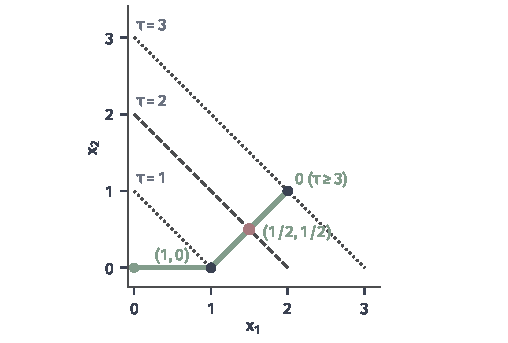
\includegraphics[width=86mm]{figures/05-optimization/06-constrained-optimization/matplotlib/sens-activeset-path/figure.pdf}
 \caption{最优解$\bm{x}^\star(\tau)$在平面上的路径（绿线）。虚线与点线是几条预算线，黑点是活动集改变的位置，红点是$\tau=2$的解。绿色文字是各段上解对$\tau$的导数：第一段$(1,0)$，第二段$(1/2,1/2)$，$\tau\geq3$时为零。}
 \label{fig:sens-activeset-path}
\end{BookInlineFigure}

$\tau=1$处，$x_2\geq0$刚要失去作用，$\lambda_3=0$。$\tau=3$处，预算刚要失去作用，$\lambda_1=0$。两处都有活动约束的乘子等于零，严格互补恰好在连接点失败。

解在连接点连续但不可微。$\tau=1$处的左导数和右导数分别是
\[
 \bm{x}'(1^-)=(1,0),\qquad\bm{x}'(1^+)=\Bigl(\frac12,\frac12\Bigr).
\]
值函数却不一样。两段的$V'$在$\tau=1$处都等于$-1$，在$\tau=3$处都等于$0$，所以$V$在连接点可微，只是二阶导数有跳跃。原因是$V'=-\lambda_1$，而$\lambda_1$连续穿过连接点：进入或离开活动集的约束，它的乘子在那里恰好是零，不造成$\lambda_1$的跳变。

\begin{BookInlineFigure}
 \centering
 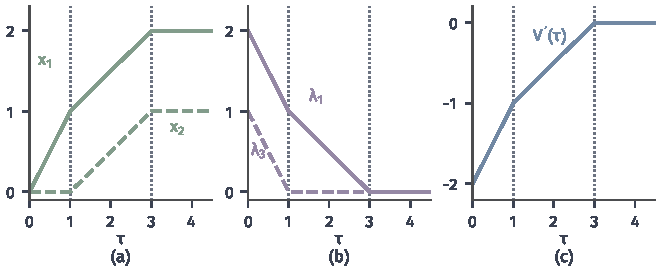
\includegraphics[width=112mm]{figures/05-optimization/06-constrained-optimization/matplotlib/sens-activeset-curves/figure.pdf}
 \caption{预算例各量随$\tau$的变化，灰色点线标出$\tau=1,3$。(a)~解的两个分量（实线$x_1$，虚线$x_2$）在连接点转折。(b)~乘子$\lambda_1$（实线）、$\lambda_3$（虚线）连续，但斜率改变。(c)~$V'(\tau)$连续，说明$V$在连接点仍然可微。}
 \label{fig:sens-activeset-curves}
\end{BookInlineFigure}

\paragraph{固定活动集的公式不能外推}
公式必须限定在它的区间内使用。把活动集$\{1\}$的公式用到$\tau=0.5$，得到$x_2=-0.25$，不可行。用到$\tau=4$，得到$\lambda_1=-1/2$，乘子符号错误。这两种错误恰好给出判别方法：预测的不活动约束是否越界，预测的乘子是否变负。

连接点上只有单侧的导数。向哪一侧走，就要换用那一侧的活动集重新写方程，上面的$\bm{x}'(1^-)$和$\bm{x}'(1^+)$正是这样得到的。

\subsection{全局最优解切换}
\label{sec:sens-global-switch}

\paragraph{两个候选的比较}
活动集改变时解连续地走过连接点。全局最优解还可能在两个相距很远的候选之间跳动。最简单的例子是在两点集合上选最小：
\begin{equation}
 \min_{x\in\{-1,1\}}\ \theta x.
 \label{eq:sens-two-points}
\end{equation}
把两个候选分别看成两条分支：
\[
 x=1:\quad v_1(\theta)=\theta,\qquad\qquad
 x=-1:\quad v_2(\theta)=-\theta.
\]
每条分支上解都是常数，$\bm{x}'=0$，值是线性函数，两者都光滑。

全局最优值取两条分支的较小者，最优解集合随$\theta$的符号改变：
\begin{equation}
 V(\theta)=-\lvert\theta\rvert,\qquad
 \bm{S}(\theta)=\begin{cases}\{1\},&\theta<0,\\\{-1,1\},&\theta=0,\\\{-1\},&\theta>0.\end{cases}
 \label{eq:sens-switching}
\end{equation}

图~\ref{fig:sens-switching}分别显示了三件事。每条分支在$\theta=0$处都很光滑。全局值在$\theta=0$处不可微。解集合在$\theta=0$处从一个点变成两个点，再变回另一个点，选出的解不连续。

\begin{BookInlineFigure}
 \centering
 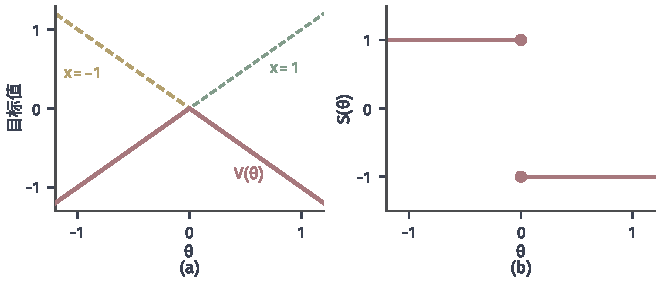
\includegraphics[width=112mm]{figures/05-optimization/06-constrained-optimization/matplotlib/sens-switching/figure.pdf}
 \caption{在$\{-1,1\}$上最小化$\theta x$。(a)~绿色虚线是$x=1$分支的值，黄色虚线是$x=-1$分支的值，红线是全局最优值$-\lvert\theta\rvert$。(b)~全局最优解集合，$\theta=0$处两个点都最优，解在此跳跃。}
 \label{fig:sens-switching}
\end{BookInlineFigure}

\paragraph{三个对象分别的结论}
定理~\ref{thm:sens-danskin}在这里成立：$\bm{C}=\{-1,1\}$是紧集，$\partial f/\partial\theta=x$连续。在$\theta=0$处，它给出
\[
 V'(0;d)=\min_{x\in\{-1,1\}}xd=-\lvert d\rvert,
\]
这与$V(\theta)=-\lvert\theta\rvert$一致。

把一条分支的导数推广成全局公式是常见的错误。$x=1$分支的导数在$\theta>0$时仍然是$1$，但$\theta>0$时全局最优解已经是$-1$，全局值的导数是$-1$。第~\ref{sec:sens-problems}节的双谷目标在连续变量上重现了同样的现象：每个谷底都有光滑的分支，全局最优解在$\theta=0$处跳到另一个谷底。在双谷的右侧分支上，驻点方程$4x^3-4x+\theta=0$对$x$的导数在$x=1$处是$8$，隐函数定理给出
\[
 x'(0)=-\frac{1}{8}.
\]
这个导数描述的是右侧谷底的移动，与全局最优解在$\theta=0$处的跳跃无关。

\subsection{退化与变化尺度}
\label{sec:sens-degeneracy}

前两种失效换了方程或换了分支。第三种失效中方程和分支都没有换，解甚至唯一，只是线性化之后的方程退化了。

\paragraph{唯一解也可能没有有限导数}
考虑
\begin{equation}
 \min_{x\in\mathbb{R}}\ \frac14x^4-\theta x.
 \label{eq:sens-quartic}
\end{equation}
对每个$\theta$，目标严格凸且强制，最优解唯一。驻点方程$x^3=\theta$给出
\[
 x^\star(\theta)=\theta^{1/3}.
\]

$\theta=0$处$x^\star=0$，Hessian$3x^2$等于零，隐函数定理的条件不成立。真实导数是
\[
 \frac{\mathrm{d}x^\star}{\mathrm{d}\theta}=\frac{1}{3\theta^{2/3}}\quad(\theta\neq0),
\]
$\theta\to0$时趋于$+\infty$，解函数在$\theta=0$处有竖直的切线。参数变化$10^{-6}$，解移动$10^{-2}$，一万倍的放大，见图~\ref{fig:sens-quartic}(b)。

值函数却没有这个问题。把解代入，
\[
 V(\theta)=\frac14\theta^{4/3}-\theta^{4/3}=-\frac34\lvert\theta\rvert^{4/3},
\]
并且$V'(\theta)=-\theta^{1/3}$，在$\theta=0$处等于零。这正是包络关系：$\partial f/\partial\theta=-x$，只需知道解的位置，不需要它的导数。再一次看到，值比解更稳定。

\begin{BookInlineFigure}
 \centering
 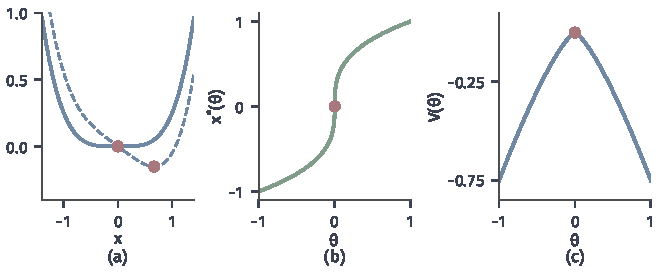
\includegraphics[width=112mm]{figures/05-optimization/06-constrained-optimization/matplotlib/sens-quartic/figure.pdf}
 \caption{退化的唯一最优解。(a)~目标$x^4/4-\theta x$，实线$\theta=0$，虚线$\theta=0.3$，红点是最小点。$\theta=0$时谷底二阶平坦。(b)~最优解$\theta^{1/3}$在$\theta=0$处切线竖直。(c)~最优值$-\tfrac34\lvert\theta\rvert^{4/3}$在$\theta=0$处可微。}
 \label{fig:sens-quartic}
\end{BookInlineFigure}

\paragraph{非退化时的放大倍数}
矩阵$\bm{K}$可逆但接近奇异时，导数存在却很大。记$\bm{z}=(\bm{x},\bm{w})$，$\bm{B}=\bm{D}_{\bm{\theta}}\bm{F}$。由式~\eqref{eq:sens-inequality-derivative}，一阶变化满足$\bm{K}\Delta\bm{z}=-\bm{B}\Delta\bm{\theta}$，因此
\begin{equation}
 \lVert\Delta\bm{z}\rVert_2\leq\lVert\bm{K}^{-1}\rVert_2\,\lVert\bm{B}\Delta\bm{\theta}\rVert_2.
 \label{eq:sens-amplification}
\end{equation}
$\lVert\bm{K}^{-1}\rVert_2$越大，同样的参数变化引起的解和乘子的变化可能越大。下面两种几何情形都会使它变大。

第一种是约束接近平行。取两条等式约束
\[
 x_1+x_2=\tau,\qquad x_1+(1+\varepsilon)x_2=2+\varepsilon.
\]
解由它们的交点确定，$\tau=2$时交点是$(1,1)$。解线性方程，得到
\[
 \bm{x}'(\tau)=\Bigl(\frac{1+\varepsilon}{\varepsilon},\ -\frac{1}{\varepsilon}\Bigr).
\]

$\varepsilon=0.25$时导数是$(5,-4)$，$\varepsilon=0.01$时是$(101,-100)$。约束梯度仍然线性无关，LICQ成立，只是接近失效。图~\ref{fig:sens-amplification}(a)里，预算线只平移一点，交点却沿着两条线滑过很长的距离。

第二种是碗的底部很平。考虑二次目标
\[
 f(\bm{x},\bm{b})=\frac12\bm{x}^{\top}\bm{H}\bm{x}-\bm{b}^{\top}\bm{x},\qquad\bm{H}=\operatorname{diag}(1,0.1).
\]
把$b_2$从$0.1$改为$0.2$，解从$(1,1)$移到$(1,2)$。参数只变化$0.1$，解移动了$1$，放大倍数是曲率的倒数，即$10$。

\begin{BookInlineFigure}
 \centering
 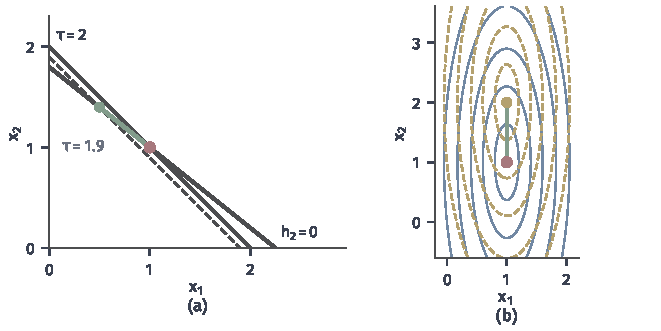
\includegraphics[width=112mm]{figures/05-optimization/06-constrained-optimization/matplotlib/sens-amplification/figure.pdf}
 \caption{两种放大机制。(a)~$\varepsilon=0.25$的两条等式约束，预算线从实线$\tau=2$平移到虚线$\tau=1.9$，交点沿绿色线段从红点移到绿点，距离约是平移量的$6.4$倍。(b)~$\bm{H}=\operatorname{diag}(1,0.1)$的目标等高线，蓝色实线是$b_2=0.1$，黄色虚线是$b_2=0.2$，最小点沿绿色线段从红点移到黄点。}
 \label{fig:sens-amplification}
\end{BookInlineFigure}

\paragraph{固有敏感性与数值误差}
上面的放大是问题的性质，与用什么算法无关。这里有两种不同的误差，需要分开。

\begin{BookInlineTable}
 \centering
 \begin{tabular}{lll}
  \toprule
  & 固有敏感性 & 数值误差\\
  \midrule
  比较 & 不同参数的精确解 & 同一问题的计算解与精确解\\
  度量 & $\bm{D}\bm{z}$的大小 & 残差、舍入与条件数\\
  改善 & 改变模型或数据 & 改进算法与精度\\
  \bottomrule
 \end{tabular}
 \caption{固有敏感性与数值误差的比较。两者都可能与$\bm{K}$的病态有关，但回答不同的问题。}
 \label{tab:sens-inherent-numerical}
\end{BookInlineTable}

矩阵的条件数大，并不一定说明解对参数敏感。把预算例中预算约束整体乘以$s>0$，写成$s(x_1+x_2-\tau)\leq0$。这是同一个约束，解不变，解对$\tau$的导数也不变，乘子则变成原来的$1/s$。相应的KKT矩阵是
\[
 \bm{K}_s=\begin{bmatrix}1&0&s\\0&1&s\\s&s&0\end{bmatrix}.
\]
$s=1$时条件数是$2$。$s=1000$时条件数约为$1415$，而$\bm{x}'(\tau)$仍然是$(1/2,1/2)$。这里的条件数变大只反映约束的书写尺度，解的敏感性没有任何变化。

解读式~\eqref{eq:sens-amplification}之前，应该先把变量和约束调整到量纲合理的尺度，计算时也应该作相应的平衡处理。只有这样，$\bm{K}$的病态才能反映问题真实的敏感性。

\section{导数的计算与核验}
\label{sec:sens-computation}

局部导数的公式已经有了，怎样计算它们，又怎样确认算出的结果可信？

\paragraph{主要思想：一次分解，多个右端}
式~\eqref{eq:sens-inequality-derivative}的系数矩阵$\bm{K}$只依赖基准点，右端$\bm{B}$的每一列对应一个参数。记$N=n+a+p$，把待求的两块Jacobian矩阵合写成
\[
 \bm{Z}=\begin{bmatrix}\bm{D}_{\bm{x}}\\\bm{D}_{\bm{w}}\end{bmatrix}\in\mathbb{R}^{N\times q}.
\]
需要解的是
\begin{equation}
 \bm{K}\bm{Z}=-\bm{B}.
 \label{eq:sens-compute}
\end{equation}
这相当于同一个矩阵配上$q$个右端，只需分解一次，然后对每一列回代。不需要对每个参数重解一次原来的非线性问题。$\bm{K}$对称而不定，通常用带主元选取的$\bm{L}\bm{D}\bm{L}^{\top}$分解，分解的做法可参考\BookChapterRef{chap:direct-linear-solvers}{卷二第12章“线性方程的直接求解”}。

分解还可以顺便检查极小性。$\bm{J}$行满秩时，$\bm{W}$在$\ker\bm{J}$上正定，当且仅当$\bm{K}$恰有$n$个正特征值、$a+p$个负特征值、没有零特征值。这称为\term{惯性}（inertia）判别，证明可查阅\scite{math-nocedal2006numerical}。$\bm{L}\bm{D}\bm{L}^{\top}$分解的$\bm{D}$与$\bm{K}$合同，读出$\bm{D}$的正负特征值个数，就得到惯性，不必另算。

\paragraph{主要思想：只要一个输出时用伴随}
有时我们并不需要整个$\bm{D}_{\bm{x}}$，只要一个标量输出$\phi(\bm{x}(\bm{\theta}))$对$q$个参数的梯度。这时梯度是
\[
 \nabla_{\bm{\theta}}\phi=\bm{D}_{\bm{x}}^{\top}\bm{c},\qquad\bm{c}=\nabla\phi(\bm{x}).
\]
代入式~\eqref{eq:sens-compute}，并在$\bm{c}$后面补零以匹配维数，就是
\begin{equation}
 \nabla_{\bm{\theta}}\phi=-\bm{B}^{\top}\bm{r},\qquad
 \bm{K}\bm{r}=\begin{bmatrix}\bm{c}\\\bm{0}\end{bmatrix}.
 \label{eq:sens-adjoint}
\end{equation}

这里用到$\bm{K}$对称。式~\eqref{eq:sens-adjoint}只解一个线性方程，与参数个数无关。这种做法称为\term{伴随法}（adjoint method）。两种算法的差别只是矩阵乘积$\bm{c}^{\top}\bm{K}^{-1}\bm{B}$的结合顺序不同，见图~\ref{fig:sens-forward-adjoint}。

\begin{BookInlineFigure}
 \centering
 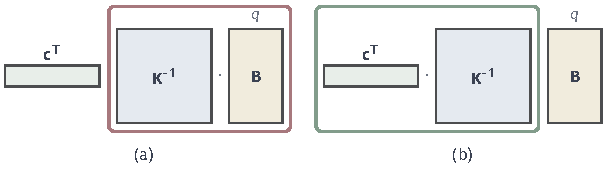
\includegraphics[width=103mm]{figures/05-optimization/06-constrained-optimization/tikz/sens-forward-adjoint/figure.pdf}
 \caption{同一乘积$\bm{c}^{\top}\bm{K}^{-1}\bm{B}$的两种结合顺序。(a)~先算红框内的$\bm{K}^{-1}\bm{B}$，每个参数一个右端，得到全部的$\bm{D}_{\bm{x}}$。(b)~先算绿框内的$\bm{c}^{\top}\bm{K}^{-1}$，只有一个右端，得到单个输出对全部参数的梯度。}
 \label{fig:sens-forward-adjoint}
\end{BookInlineFigure}

表~\ref{tab:sens-cost}比较各种做法的成本，规模变量为$N$与$q$，运算量只计首项。重新求解一列的成本指做一次完整的$\bm{K}$分解，实际的非线性重解通常更贵。$\bm{K}$稀疏时，分解成本由消元产生的填充决定，回代成本是$\bm{L}$的非零元个数的两倍，表中的立方、平方相应缩小，分解一次多次回代的比例关系不变。

\begin{BookInlineTable}
 \centering
 \begin{tabular}{lll}
  \toprule
  做法 & 稠密运算量 & 得到什么\\
  \midrule
  每个参数重解 & $qN^3/3$ & 全部$\bm{D}_{\bm{x}}$\\
  一次分解，$q$次回代 & $N^3/3+2qN^2$ & 全部$\bm{D}_{\bm{x}}$和$\bm{D}_{\bm{w}}$\\
  伴随法 & $N^3/3+2N^2$ & 一个输出的梯度\\
  \bottomrule
 \end{tabular}
 \caption{计算解对参数导数的稠密运算量，$N=n+a+p$。分解的复用要求活动集不变。伴随法的结果再乘$\bm{B}^{\top}$需要的运算量与$\bm{B}$的非零元个数成正比。}
 \label{tab:sens-cost}
\end{BookInlineTable}

\paragraph{计算过程}
下面把全过程用在一个小例子上。预算例中同时考虑两个参数，预算$\tau$和理想点的横坐标偏移$\theta$，基准是$(\tau,\theta)=(2,0)$，目标是
\[
 f(\bm{x},\theta)=\frac12(x_1-2-\theta)^2+\frac12(x_2-1)^2.
\]

\needspace{6\baselineskip}
\paragraph{变量}
\begin{itemize}
 \item 基准解$\bm{x}\in\mathbb{R}^n$，活动乘子与等式乘子合写成$\bm{w}\in\mathbb{R}^{a+p}$。
 \item 系数矩阵$\bm{K}\in\mathbb{R}^{N\times N}$，右端$\bm{B}\in\mathbb{R}^{N\times q}$，$N=n+a+p$。
 \item 输出$\bm{Z}$，形状是$N\times q$，含$\bm{D}_{\bm{x}}$与$\bm{D}_{\bm{w}}$两块。
 \item 每个不活动约束的余量，每个活动约束的乘子，它们决定分支的有效范围。
\end{itemize}

\paragraph{初始化}
先把基准问题求解到足够高的精度，读出解和乘子，再分出活动约束。

例中$n=2$，$a=1$，$p=0$，$q=2$。基准解和乘子是
\[
 \bm{x}=\begin{bmatrix}3/2\\1/2\end{bmatrix},\qquad\lambda_1=\frac12,\qquad A=\{1\}.
\]

\paragraph{计算步骤}
\begin{enumerate}
 \item 组装$\bm{K}$和$\bm{B}$，公式见式~\eqref{eq:sens-inequality-derivative}。

 例中Lagrange函数的梯度和活动约束分别是
 \[
  \nabla_{\bm{x}}\mathcal{L}=(x_1-2-\theta+\lambda_1,\ x_2-1+\lambda_1),\quad g_1=x_1+x_2-\tau,
 \]
 对$\bm{x}$、$\lambda_1$和$(\tau,\theta)$分别求偏导，得到
 \[
  \bm{K}=\begin{bmatrix}1&0&1\\0&1&1\\1&1&0\end{bmatrix},\qquad
  \bm{B}=\begin{bmatrix}0&-1\\0&0\\-1&0\end{bmatrix}.
 \]
 $\bm{B}$的第一列对应$\tau$，第二列对应$\theta$。

 \item 分解$\bm{K}=\bm{L}\bm{D}\bm{L}^{\top}$，并由$\bm{D}$的符号检查惯性。

 例中不需要主元交换，消元得到
 \[
  \bm{L}=\begin{bmatrix}1&0&0\\0&1&0\\1&1&1\end{bmatrix},\qquad
  \bm{D}=\operatorname{diag}(1,1,-2).
 \]
 $\bm{D}$有两个正数和一个负数，与$n=2$，$a=1$相符，这个解是局部极小点。

 \item 对$\bm{B}$的每一列回代，得到$\bm{Z}$的相应列，公式见式~\eqref{eq:sens-compute}。

 例中$\tau$列的右端是$(0,0,1)^{\top}$。依次解$\bm{L}\bm{y}=(0,0,1)^{\top}$、$\bm{D}\bm{y}'=\bm{y}$、$\bm{L}^{\top}\bm{z}=\bm{y}'$，中间结果和最终结果是
 \[
  \bm{y}=\begin{bmatrix}0\\0\\1\end{bmatrix},\quad
  \bm{y}'=\begin{bmatrix}0\\0\\-1/2\end{bmatrix},\quad
  \bm{z}=\begin{bmatrix}1/2\\1/2\\-1/2\end{bmatrix}.
 \]

 $\theta$列的右端是$(1,0,0)^{\top}$，同样回代，得到
 \[
  \bm{y}=\begin{bmatrix}1\\0\\-1\end{bmatrix},\quad
  \bm{y}'=\begin{bmatrix}1\\0\\1/2\end{bmatrix},\quad
  \bm{z}=\begin{bmatrix}1/2\\-1/2\\1/2\end{bmatrix}.
 \]

 \item 用余量和乘子确定有效范围。把导数代入，对方向$(\Delta\tau,\Delta\theta)$写出需要保持为正的量。

 例中这三个量分别是
 \[
  \begin{aligned}
  \lambda_1&=\frac12-\frac12\Delta\tau+\frac12\Delta\theta,\\
  x_1&=\frac32+\frac12\Delta\tau+\frac12\Delta\theta,\\
  x_2&=\frac12+\frac12\Delta\tau-\frac12\Delta\theta.
  \end{aligned}
 \]
 它们都大于零的区域是参数平面上的一个多面体，图~\ref{fig:sens-critical-regions}中绿色的带形就是这个区域在图中范围内的部分。

 \item 给出预测，并用小幅参数重求解核验：预测的活动集是否保持，预测的解与重解的结果相差多少。

 例中取$(\Delta\tau,\Delta\theta)=(0.2,0.1)$，三个量都为正，预测和重解都是
 \[
  \bm{x}=(1.65,\ 0.55),\qquad\lambda_1=0.45.
 \]
 问题在这个活动集上是二次的，所以预测是精确的。若取$(\Delta\tau,\Delta\theta)=(-1.5,0)$，预测给出$x_2=-1/4<0$，这说明活动集已经改变，需要换到活动集$\{1,3\}$重新计算，真实解是$(0.5,0)$。
\end{enumerate}

整个计算是一次完成的，没有迭代，到步骤五结束。最终得到
\[
 \bm{D}_{\bm{x}}=\begin{bmatrix}1/2&1/2\\1/2&-1/2\end{bmatrix},\qquad
 \bm{D}_{\lambda_1}=\begin{bmatrix}-1/2&1/2\end{bmatrix}.
\]

\begin{BookInlineFigure}
 \centering
 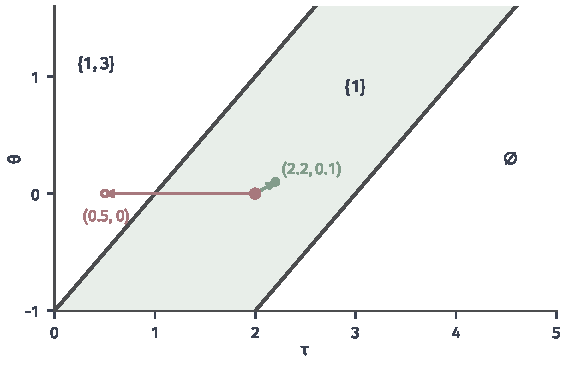
\includegraphics[width=96mm]{figures/05-optimization/06-constrained-optimization/matplotlib/sens-critical-regions/figure.pdf}
 \caption{参数平面$(\tau,\theta)$上的活动集区域。两条深灰线是$\tau=1+\theta$和$\tau=3+\theta$，它们划分出活动集$\{1,3\}$、$\{1\}$和$\varnothing$。红点是基准$(2,0)$，绿色箭头走到同一区域内的$(2.2,0.1)$，一阶预测有效；红色箭头越过边界到$(0.5,0)$，一阶预测失效。}
 \label{fig:sens-critical-regions}
\end{BookInlineFigure}

伴随法在这个例子上也可以手算。设只关心输出$\phi=x_2$，$\bm{c}=(0,1)^{\top}$。由式~\eqref{eq:sens-adjoint}，解$\bm{K}\bm{r}=(0,1,0)^{\top}$，得到$\bm{r}=(-1/2,1/2,1/2)^{\top}$，再求
\[
 \nabla_{(\tau,\theta)}x_2=-\bm{B}^{\top}\bm{r}=\begin{bmatrix}1/2\\-1/2\end{bmatrix}.
\]
这正是$\bm{D}_{\bm{x}}$的第二行，一次回代就得到了两个参数的结果。

\paragraph{算法分析：误差的三个来源}
隐式导数的公式对应精确的最优性方程。实际算出的导数还带有三种误差，它们的性质不同。

第一种是近似解带来的误差。基准解只解到$\tilde{\bm{x}}$，$\bm{K}$和$\bm{B}$都在$\tilde{\bm{x}}$处组装，导数的误差与解的误差成正比，比例系数由$\bm{K}^{-1}$和二阶导数的变化率决定。参数只出现在线性项时$\bm{B}$不依赖于$\bm{x}$，二次目标下这项误差为零。

第二种是有限差分的误差。用重解来核验导数时，常用中心差分
\[
 \frac{\bm{x}(\bm{\theta}+h\bm{d})-\bm{x}(\bm{\theta}-h\bm{d})}{2h},
\]
截断误差是$O(h^2)$。若每次重解的误差是$\varepsilon$，差分会放大成$O(\varepsilon/h)$。两项相加的误差在$h\sim\varepsilon^{1/3}$时最小，约为$\varepsilon^{2/3}$。

第三种是算法展开的误差。把迭代算法写成关于$\bm{\theta}$的函数，对$T$步迭代逐步求导，得到的是$\bm{x}^{(T)}$的导数，而不是$\bm{x}^\star$的导数。以梯度下降为例，它的迭代是
\[
 \bm{x}^{(t+1)}=\bm{x}^{(t)}-\alpha\nabla_{\bm{x}}f(\bm{x}^{(t)},\bm{\theta}),
\]
导数的递推式是
\begin{equation}
 \bm{D}^{(t+1)}=\bigl(\bm{I}-\alpha\nabla^2_{\bm{x}\bm{x}}f\bigr)\bm{D}^{(t)}-\alpha\nabla^2_{\bm{x}\bm{\theta}}f,
 \label{eq:sens-unroll}
\end{equation}
其中各导数都在$(\bm{x}^{(t)},\bm{\theta})$处取值。它的不动点正是式~\eqref{eq:sens-unconstrained-derivative}。

图~\ref{fig:sens-fd-unroll}用具体计算展示了这些误差。(a)中，差分误差先随$h$减小而减小，到某个$h$之后反而增大，这个转折点随求解精度$\varepsilon$移动。(b)在岭回归例子上比较了式~\eqref{eq:sens-unroll}的展开和在当前迭代点上计算的隐式导数：$\gamma$改变了曲率，展开的误差多了一个随$t$增长的因子，所以比隐式导数略慢。

\begin{BookInlineFigure}
 \centering
 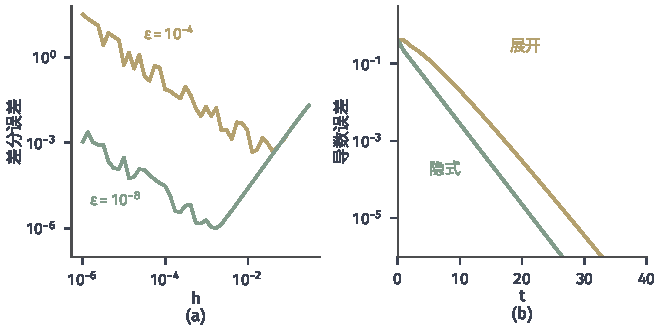
\includegraphics[width=112mm]{figures/05-optimization/06-constrained-optimization/matplotlib/sens-fd-unroll/figure.pdf}
 \caption{导数计算的误差。(a)~价格例$\theta=1$处$x_2$对$\theta$的中心差分误差。每次重解用梯度下降到残差$\varepsilon$，曲线取$40$次随机起点的中位数，黄线$\varepsilon=10^{-4}$，绿线$\varepsilon=10^{-8}$。(b)~岭回归例$\gamma=1$，步长$\alpha=1/L$，黄线是展开$t$步梯度下降得到的导数的误差，绿线是在$\bm{x}^{(t)}$处计算隐式导数的误差。}
 \label{fig:sens-fd-unroll}
\end{BookInlineFigure}

\paragraph{算法分析：非二次问题的核验}
第~\ref{sec:sens-general-constraints}节的价格例不是二次的，一阶预测有误差，可以检验误差的阶。在$\theta=1$处，由$\lambda'(1)=1$，$x_1'=1-\lambda-\lambda'\theta=-1/2$，$x_2'=-\lambda'=-1$。与重解的结果比较，
\[
 \begin{aligned}
 h&=0.1:\quad \bm{x}=(1.4480,\ 0.4072),\quad\text{预测}\ (1.45,\ 0.4),\\
 h&=0.01:\quad \bm{x}=(1.49498,\ 0.49007),\quad\text{预测}\ (1.495,\ 0.49).
 \end{aligned}
\]
误差分别约为$7.5\times10^{-3}$和$7.9\times10^{-5}$，$h$缩小十倍，误差缩小约一百倍，与二阶截断误差一致。

这个一致性只在活动集保持时成立。价格例的预算活动窗口是$(\sqrt{5}-1)/2<\theta<2$，$\theta>2$时$x_2\geq0$起作用。图~\ref{fig:sens-prediction-error}(b)中，$h$接近$1$时误差开始偏离$h^2$的规律。检验时还应比较左右两侧的差商，它们不相等，或者差商不随$h$收敛，常常说明活动集正在改变。

\begin{BookInlineFigure}
 \centering
 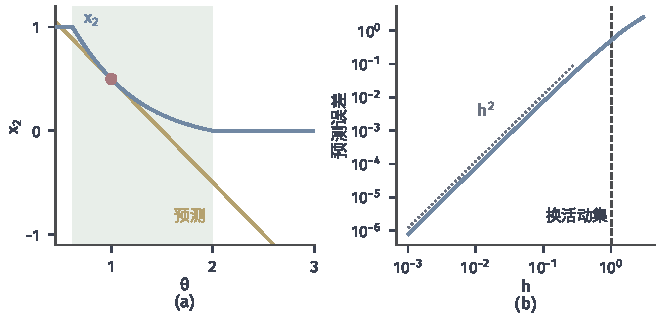
\includegraphics[width=112mm]{figures/05-optimization/06-constrained-optimization/matplotlib/sens-prediction-error/figure.pdf}
 \caption{价格例的一阶预测。(a)~$x_2(\theta)$的真实值（蓝线）和$\theta=1$处的线性预测（黄线），绿色区域是活动集保持的窗口。(b)~预测误差随$h$的变化（对数坐标，$\theta=1+h$），灰色点线是$h^2$的参考线，黑色虚线标出活动集改变的位置$h=1$。}
 \label{fig:sens-prediction-error}
\end{BookInlineFigure}

\section{本章小结}
\label{sec:sens-summary}

本章开头问：预算多一点，最优值变化多少，最优解往哪里移？回答这个问题，首先要说清比较的对象。最优值函数$V$是全局的，分支上的值$v$是局部的，解集合$\bm{S}$可能为空或含多个点，只有选定分支或选解规则才有“解的导数”可谈。

最优值的变化有两类结论。约束右端扰动时，零间隙且乘子达到就给出对任意大小的扰动都成立的仿射下界，它不要求凸性，也不要求活动集不变。只有在$V$可微时，下界的斜率才等于实际导数；$V$不可微时，全体最优乘子的相反数构成全部下界斜率，方向导数由其中最不利的一个决定。目标参数的变化由包络关系描述，一般含参约束下导数等于Lagrange函数显含参数的偏导。

最优解的移动由可逆的最优性方程描述。无约束时看Hessian，等式约束时看KKT矩阵，只需在切空间上正定。不等式约束再加上LICQ与严格互补，活动约束便可当作等式处理。隐函数定理给出的是局部结论，定理的条件是充分而非必要的，方程的光滑解也要用二阶条件判定是否极小。

这些局部结论的失效方式彼此不同。活动集改变时，解连续但转折，值函数可能仍然可微。全局最优解切换时，每条分支都光滑，全局值出现折角，解发生跳跃。方程退化时，唯一的解也可能没有有限的导数，而值函数依然可微。判别时要看的是可用的方程、所选的分支和线性方程的可逆性分别是否变化。

计算时，同一次$\bm{K}$分解可以服务多个右端，只要一个输出的梯度时伴随法只需一个右端。隐式导数对应精确的最优性方程，近似解、有限差分和有限次算法展开各自带有不同的误差，预测的有效性要靠余量、乘子符号和小幅重解来核验。第~\ref{chap:simplex-method}章的固定基分析正是这一思路在线性规划上的实例，第~\ref{chap:bilevel-optimization}章将继续用解映射的导数研究双层优化。

